
% $Id: manual_tex.tex,v 1.2 2006-10-30 20:40:21 sarich Exp $ 
%
% LATEX version of the TAO users manual.
%
% manual_tex.tex is the base file for LaTeX format, while manual.tex is
% the corresponding base HTML format file.
%
\documentclass[11pt,openright]{book}
\usepackage{epsf}
\usepackage{amssymb}
\usepackage{amsfonts}
\usepackage{amsmath}
\usepackage{geometry}

% moreverb provides commands for reading and writing files. In particular,
% verbatiminput. See pages 66-70 on the LateX Companion.
\usepackage{moreverb}

% float supersedes the obsolete here package. See page 149 of the 
% LateX Companion.
\usepackage{float}

% url is a form of \verb intended for addresses, hypertext links, 
% directories/paths,...
\usepackage{url}
\usepackage{pdfpages}
\usepackage[bookmarksopen,colorlinks]{hyperref}

% afterpage places documents at the top of the page. See page 150 of the 
% LateX Companion.
\usepackage{afterpage}

\setlength{\textwidth}{6.0in}
\setlength{\oddsidemargin}{18pt}
\setlength{\evensidemargin}{18pt}
\setlength{\topmargin}{-0.5in}
\setlength{\textheight}{8.5in}

\newcommand{\half}{{\textstyle{\frac{1}{2}}}}
\newcommand{\findex}[1]{\index{#1}}
\newcommand{\sindex}[1]{\index{#1}}
\newcommand{\F}{\mbox{\boldmath \(F\)}}
\newcommand{\x}{\mbox{\boldmath \(x\)}}
\newcommand{\rr}{\mbox{\boldmath \(r\)}}
\newcommand{\R}{\mathbb R}
\renewcommand{\Re}{\R}
\newcommand{\Comment}[1]{}

\makeindex
 
% Defines the environment where design issues are discussed. In the manual
% version of this report, these regions are ignored.
\def\design{\medskip \noindent Design Issue:\begin{em}}
\def\enddesign{\end{em} \medskip}

% Print DRAFT in large letters across every page
%\special{!userdict begin /bop-hook{gsave 200 70 translate
%65 rotate /Times-Roman findfont 216 scalefont setfont
%0 0 moveto 0.95 setgray (DRAFT) show grestore}def end}

\begin{document}
\pagestyle {empty}


%\pagestyle {empty}
%\includepdf[pages={1,2,3}]{ANL-MCS-TM-322.pdf}

\pagestyle{empty}
\hspace{-.65in}
\includegraphics{ArgonneLogo}
\hfill  {\large {\bf ANL/MCS-TM-322 Rev. 3.14}}

\vspace*{2in}
\noindent {\huge{\bf TAO Users Manual}}
\vspace*{8pt}
\hrule
\vspace*{8pt}
\noindent {\Large{\it Revision 3.14}}

\vspace*{1in}
\noindent \\
{\Large {\bf Mathematics and Computer Science Division}}

\vspace*{10pt}


\vspace*{20pt}

%%%%%%%%%%%%%%%%%%%%%%%%%%%%%%%%%%%%%%%%%%%%%%%%%%%%%%%%%%%%%%%%%%%%%%%%%%%%%%%%%%%%

\newpage
\newgeometry{top=0mm, left=0mm, right=0mm, bottom=0mm}
\centerline{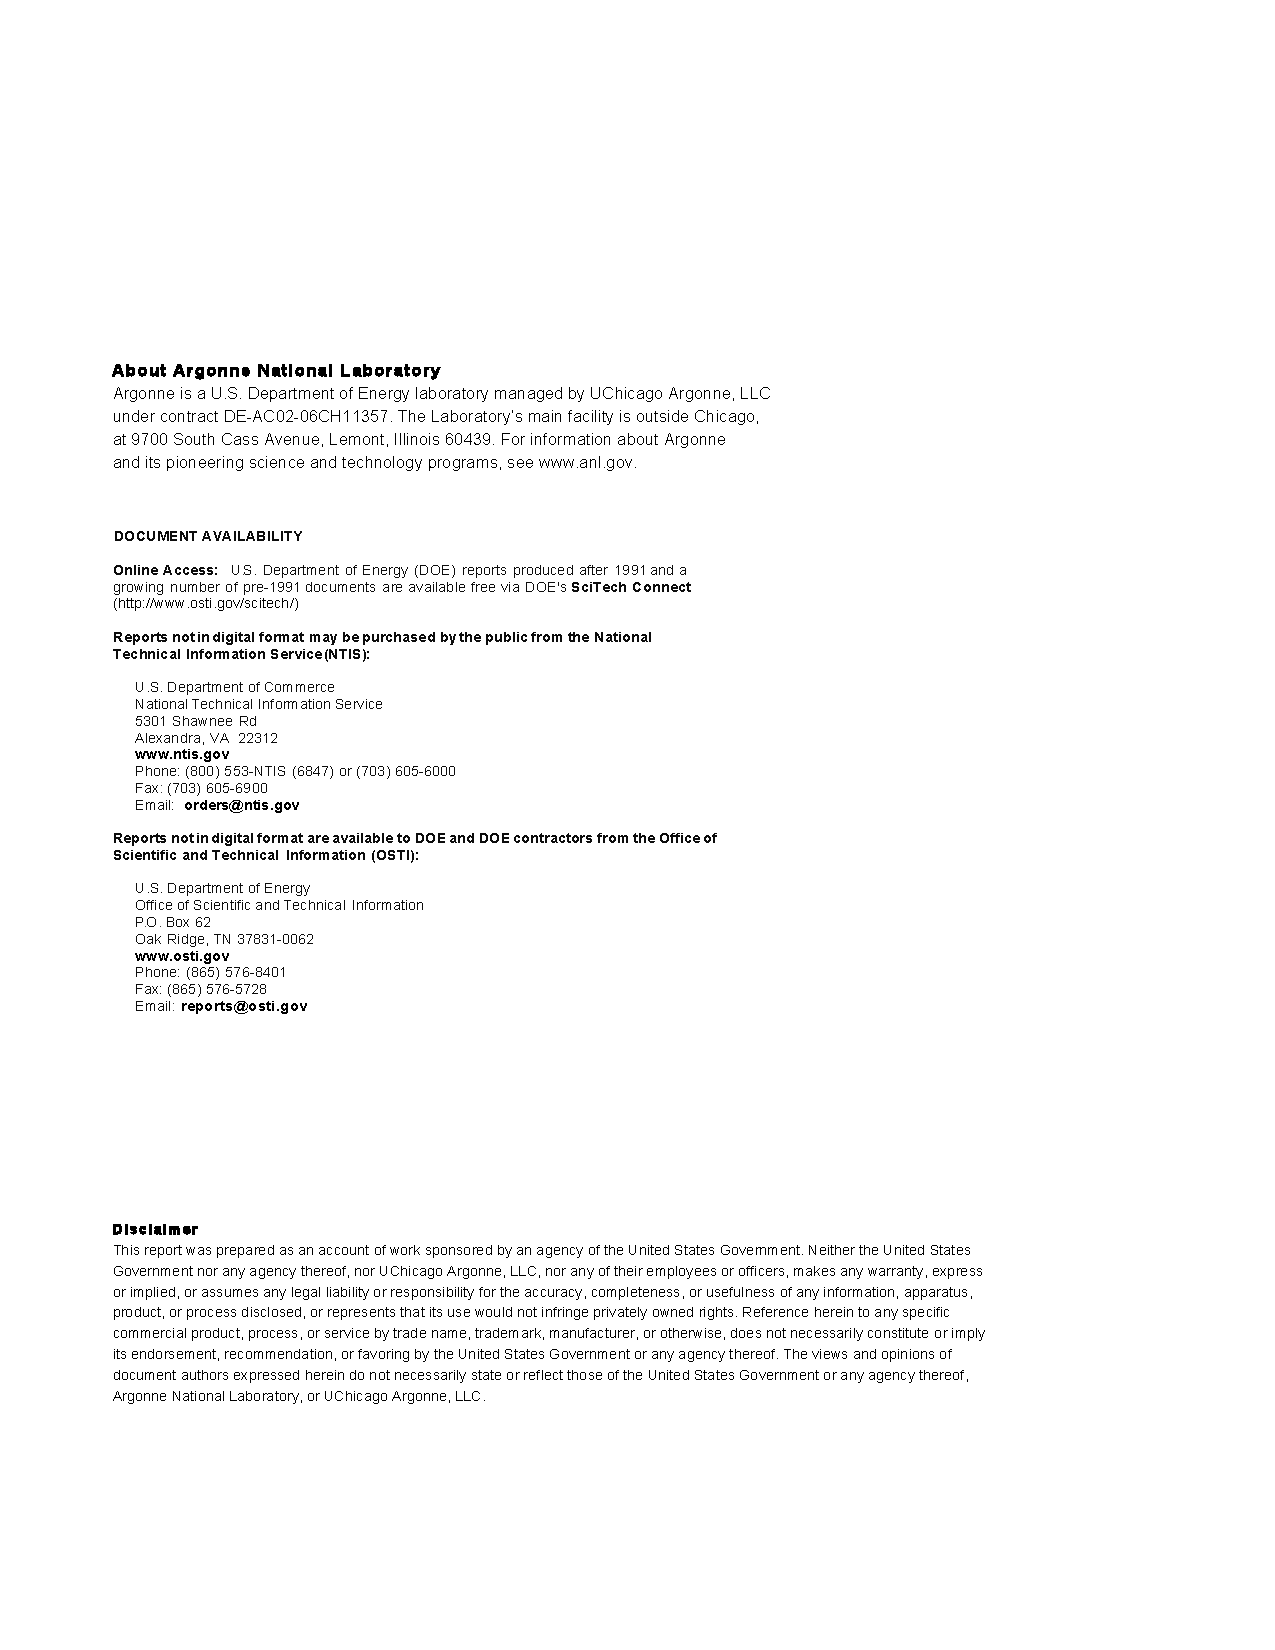
\includegraphics{ArgonneReportTemplatePage2}}
\newpage
\restoregeometry

%%%%%%%%%%%%%%%%%%%%%%%%%%%%%%%%%%%%%%%%%%%%%%%%%%%%%%%%%%%%%%%%%%%%%%%%%%%%%%%%%%%%

\pagestyle{empty}
\hfill {\large {\bf ANL/MCS-TM-322 Rev. 3.14}}

\vspace*{2in}
\noindent {\LARGE{\bf TAO Users Manual}}
\vspace*{8pt}
\hrule
\vspace*{8pt}
\noindent {\Large{\it Revision 3.14}}

\vspace*{0.5in}
\noindent Prepared by \\
{\bf Alp Dener \\ Adam Denchfield \\ Hansol Suh \\ Todd Munson \\ Jason Sarich \\ Stefan Wild \\ Steven Benson \\ Lois Curfman McInnes}\\

\vspace*{30pt}
\noindent September 2020

\vspace*{20pt}
\noindent This work was supported by the Office of Advanced Scientific Computing Research, \\
Office of Science, U.S. Department of Energy, under Contract DE-AC02-06CH11357.


% Table of contents.
\cleardoublepage
\pagestyle {plain}
\pagenumbering{roman}
\setcounter{page}{1}
\tableofcontents

\cleardoublepage
\input{abstract.tex}
\input{changes.tex}
\input{acknowl.tex}

\cleardoublepage
\input{license.tex}

% Start of the Users Manual
\cleardoublepage
\setcounter {page}{1}
\pagenumbering{arabic}

\input{part0.tex}
\chapter{Getting Started}
\label{chapter_intro_tao}

TAO can be used on a personal
computer with a single processor or within a parallel environment.  
Its basic usage involves only a few commands, but fully 
understanding its usage requires time.
Application programmers can easily begin to use TAO by working with 
the examples provided and then gradually learn more details according to
their needs.  The current version of TAO and the most recent help 
concerning installation and usage can be found at  
\url{https://www.mcs.anl.gov/research/projects/tao/}.

See the PETSc users manual and \url{https://www.mcs.anl.gov/petsc} for how to install and start using PETSc/TAO.

\section{Writing Application Codes with TAO}

Examples throughout the library demonstrate the software usage and
can serve as templates for developing custom applications.  We suggest
that new TAO users examine programs in
\begin{verbatim}
   ${PETSC_DIR}/src/tao/<unconstrained,bound,..>/tutorials.
\end{verbatim} 
The HTML version of the manual pages located at
\begin{verbatim}
   ${PETSC_DIR}/docs/manpages/index.html
\end{verbatim} % To fool the coloring algorithm $
\noindent
and
\begin{verbatim}
   https://www.mcs.anl.gov/petsc/documentation/index.html
\end{verbatim}
\noindent
provides indices (organized by both routine names and concepts) to the
tutorial examples.

We suggest the following procedure for writing a new application
program using TAO:

\begin{enumerate}
\item Install PETSc/TAO according to the instructions in
  \url{https://www.mcs.anl.gov/petsc/documentation/installation.html}.
\item Copy an example and makefile from the directories
\begin{verbatim}
   ${PETSC_DIR}/src/tao/<unconstrained,bound,..>/tutorials.
\end{verbatim} 
  compile the example, and run the program. 
\item Select the example program matching the application most
  closely, and use it as a starting point for developing a customized
  code.
\end{enumerate}

\section{A Simple TAO Example}
\label{sec_simple}

To help the user start using TAO immediately, we introduce here a simple
uniprocessor example. Please read Section~\ref{chapter_tao_solver} for a 
more in-depth discussion on using the TAO solvers.
The code presented in Figure~\ref{fig:example1} minimizes the
extended Rosenbrock function $f: \Re^n \to \Re$ defined by
\[
 f(x) = 
 \sum_{i=0}^{m-1} \left( \alpha(x_{2i+1}-x_{2i}^2)^2 + (1-x_{2i})^2 \right),
\]
where $n = 2m$ is the number of variables.  Note that while we use the C 
language to introduce the TAO software, the package is fully usable from 
C++ and Fortran77/90.  Section~\ref{chapter_fortran} discusses additional 
issues concerning Fortran usage.

\afterpage{
\begin{figure}[H]
  {\footnotesize \verbatiminput{rosenbrock1.c}}
\caption{Example of Uniprocessor TAO Code\label{fig_example1}}
\end{figure}
}


The code in Figure~\ref{fig_example1} contains many of the components
needed to write most TAO programs and thus is illustrative of the
features present in complex optimization problems.  Note that for
display purposes we have omitted some nonessential lines of code as well as the
(essential) code required for the routine \texttt{FormFunctionGradient},
which evaluates the function and gradient, and the code for
\texttt{FormHessian}, which evaluates the Hessian matrix for Rosenbrock's
function. The complete code is available in \url{$TAO\_DIR/src/unconstrained/tutorials/rosenbrock1.c}. %$
The following sections annotates the lines of code in
Figure~\ref{fig_example1}.

\section{Include Files}

The include file for TAO should be used via the statement
\begin{verbatim}
   #include <petsctao.h>
\end{verbatim}
\noindent
The required lower-level include files are automatically included
within this high-level file.

\section{TAO Solvers}

Many TAO applications will follow an ordered set of procedures for 
solving an optimization problem:
The user creates a \texttt{Tao} context and selects a default algorithm. 
Call-back routines as well as vector (\texttt{Vec}) and matrix (\texttt{Mat}) 
data structures are then set.  These call-back routines will be used for 
evaluating the objective function, gradient, and perhaps the Hessian 
matrix.  The user then invokes TAO to solve the optimization problem and 
finally destroys
the \texttt{Tao} context. A list of the necessary functions for 
performing these steps
using TAO are shown in Figure \ref{fig_tao_commands}.  Details of these commands are presented in
Chapter~\ref{chapter_tao_solver}.

\findex{TaoCreate()} \findex{TaoSetObjectiveAndGradientRoutine()}
\findex{TaoSetRoutine()} \findex{TaoSolve()}
\findex{TaoDestroy()} \findex{TaoSetInitialVector()}
\begin{figure}[H]
\begin{verbatim}
   TaoCreate(MPI_Comm comm, Tao *tao); 
   TaoSetType(Tao tao, TaoType type);
   TaoSetInitialVector(Tao tao, Vec x);
   TaoSetObjectiveAndGradientRoutine(Tao tao, 
        PetscErrorCode (*FormFGradient)(Tao,Vec,PetscReal*,Vec,void*), 
        void *user);
   TaoSetHessianRoutine(Tao tao, Mat H, Mat Hpre,
        PetscErrorCode (*FormHessian)(Tao,Vec,Mat,Mat,
        void*), void *user);
   TaoSolve(Tao tao);
   TaoDestroy(Tao tao);
\end{verbatim}
\caption{Commands for Solving an Unconstrained Optimization Problem
\label{fig_tao_commands}}
\end{figure}

Note that the solver algorithm selected through the function 
\texttt{TaoSetType()} can be overridden
at runtime by using an options database.  Through this
database, the user not only can select a minimization method (e.g.,
limited-memory variable metric, conjugate gradient, Newton with line
search or trust region) but also can prescribe the convergence
tolerance, set various monitoring routines, set iterative methods
and preconditions for solving the linear systems, and so forth.  See 
Chapter~\ref{chapter_tao_solver} for more information on the 
solver methods available in TAO.

\section{Function Evaluations}

Users of TAO are required to provide routines that perform function
evaluations. Depending on the solver chosen, they may also have to
write routines that evaluate the gradient vector and Hessian matrix.

\section{Programming with PETSc}
\label{sec_tao_programming}
TAO relies heavily on PETSc not only for its vectors, matrices, and linear
solvers but also for its programming utilities such as command line option 
handling, error handling, and compiling system.  We provide here a quick 
overview of some of these PETSc features.  Please refer to the PETSc 
manual \cite{petsc-user-ref} for a more in-depth
discussion of PETSc.

\subsection*{Vectors}

In the example in Figure \ref{fig_example1}, the vector data structure
(\texttt{Vec}) is used to store the solution and gradient for the TAO
unconstrained minimization solvers.  A new parallel or sequential
vector \texttt{x} of global dimension \texttt{M} is created with the
command 
\begin{verbatim}
   info = VecCreate(MPI_Comm comm,int m,int M,Vec *x);
\end{verbatim}
\noindent
where \texttt{comm} denotes the MPI communicator. The type of storage
for the vector may be set with calls either to \texttt{VecSetType()}
or to \texttt{VecSetFromOptions()}.  Additional vectors of the same type
can be formed with 
\begin{verbatim}
   info = VecDuplicate(Vec old,Vec *new);
\end{verbatim}
\noindent
The commands
\begin{verbatim}
   info = VecSet(Vec X,PetscScalar value);
   info = VecSetValues(Vec x,int n,int *indices,
                       Scalar *values,INSERT_VALUES);
\end{verbatim}
\noindent
respectively set all the components of a vector to a particular scalar
value and assign a different value to each component.  More detailed
information about PETSc vectors, including their basic operations,
scattering/gathering, index sets, and distributed arrays, may be found
in the PETSc users manual \cite{petsc-user-ref}.

\subsection*{Matrices}

Usage of matrices and vectors is similar. \sindex{matrix} 
The user can create a new parallel or sequential matrix \texttt{H} with 
\texttt{M} global rows and \texttt{N} global columns, with the routines

\begin{verbatim}
   ierr = MatCreate(MPI_Comm comm,Mat *H);
   ierr = MatSetSizes(H,PETSC_DECIDE,PETSC_DECIDE,M,N);
\end{verbatim}
\noindent
where the matrix format can be specified at runtime.  The user could
alternatively specify each processes's number of local rows and columns
using \texttt{m} and \texttt{n} instead of \texttt{PETSC\_DECIDE}.  
\texttt{H} can then be used to store
the Hessian matrix, as indicated by the call to
\texttt{TaoSetHessianMat()}.  Matrix entries can be set with the
command
\begin{verbatim}
   ierr = MatSetValues(Mat H,PetscInt m,PetscInt *im, PetscInt n,
                       PetscInt *in, PetscScalar *values,INSERT_VALUES);
\end{verbatim}
\noindent
After %\findex{MatSetValues()} 
all elements have been inserted into the
matrix, it must be processed with the pair of commands

\begin{verbatim}
   ierr = MatAssemblyBegin(Mat H,MAT_FINAL_ASSEMBLY);
   ierr = MatAssemblyEnd(Mat H,MAT_FINAL_ASSEMBLY);
\end{verbatim}
\noindent
The PETSc users manual \cite{petsc-user-ref} discusses
various matrix formats as
well as the details of some basic matrix manipulation routines.


\subsection*{The Options Database}
\label{sec_options}
A TAO application can access the command line options presented at
runtime through the PETSc options database. This database gives the application
author the ability to set and change application parameters without
the need to recompile the application. For example, 
an application may have a grid discretization parameter \texttt{nx}
that can be set with the command line option \texttt{-nx <integer>}.
The application can read this option with the following line of code:
\begin{verbatim}
   PetscOptionsGetInt(NULL,NULL, "-nx", &nx, &flg);
\end{verbatim}
\noindent
If the command line option is present, the variable \texttt{nx} is set
accordingly; otherwise, \texttt{nx} remains unchanged. A complete
description of the options database may be found in the PETSc users
manual \cite{petsc-user-ref}.

\subsection*{Error Checking}

All TAO commands begin with the \texttt{Tao} prefix and return an
integer indicating whether an error has occurred during the call.  The
error code equals zero after the successful completion of the routine
and is set to a nonzero value if an error has been detected.  The
macro \texttt{CHKERRQ(ierr)} checks the value of \texttt{ierr} and calls an
error handler upon error detection.  \texttt{CHKERRQ()} should be used after
all subroutines to enable a complete error traceback.

In Figure \ref{fig_traceback} we indicate a traceback generated by
error detection within a sample program. The error occurred on line
2110 of the file \texttt{\$\{PETSC\_DIR\}/src/mat/inter\-face/mat\-rix.c} in the
routine \texttt{MatMult()} and was caused by failure to assemble the 
matrix in the Hessian evaluation routine.
The \texttt{MatMult()} routine was called from
the \texttt{TaoSolve\_NLS()} routine, which was in turn called on line 
154 of \texttt{TaoSolve()} from the \texttt{main()} routine 
in the program \texttt{rosenbrock1.c}.  The PETSc users
manual \cite{petsc-user-ref} provides further details
regarding error checking, including
information about error handling in Fortran.

\begin{figure}[htb]
{\footnotesize
\begin{verbatim}
> rosenbrock1 -tao_type nls
[0]PETSC ERROR: --------------------- Error Message ------------------------------------
[0]PETSC ERROR: Object is in wrong state!
[0]PETSC ERROR: Not for unassembled matrix!
[0]PETSC ERROR: ------------------------------------------------------------------------
[0]PETSC ERROR: Petsc Development HG revision: b95ffff514b66a703d96e6ae8e78ea266ad2ca19
[0]PETSC ERROR: See docs/changes/index.html for recent updates.
[0]PETSC ERROR: See docs/faq.html for hints about trouble shooting.
[0]PETSC ERROR: See docs/index.html for manual pages.
[0]PETSC ERROR: ------------------------------------------------------------------------
[0]PETSC ERROR: Libraries linked from petsc/arch-linux2-c-debug/lib
[0]PETSC ERROR: Configure run at Tue Jul 19 14:13:14 2011
[0]PETSC ERROR: Configure options --with-shared-libraries --with-dynamic-loading
[0]PETSC ERROR: ------------------------------------------------------------------------
[0]PETSC ERROR: MatMult() line 2110 in petsc/src/mat/interface/matrix.c
[0]PETSC ERROR: TaoSolve_NLS() line 291 in src/unconstrained/impls/nls/nls.c
[0]PETSC ERROR: TaoSolve() line 154 in src/interface/tao.c
[0]PETSC ERROR: main() line 94 in src/unconstrained/tutorials/rosenbrock1.c
application called MPI_Abort(MPI_COMM_WORLD, 73) - process 0
\end{verbatim}
}
\caption{Example of Error Traceback}
\label{fig_traceback}
\end{figure}

When running the debugging version of the TAO software (PETSc configured 
with the (default) \texttt{--with-debugging} option), checking is performed for 
memory corruption
(writing outside of array bounds, etc). The macros \texttt{CHKMEMQ} and
\texttt{CHKMEMA} can be called anywhere in the code and, when used together 
with the command line option \texttt{-malloc\_debug}, check the current
status of the memory for corruption.  By putting several (or many) of
these macros into an application code, one can usually track
down the code segment where corruption has occurred.

\subsection*{Parallel Programming}

Since TAO uses the message-passing model for parallel programming and
employs MPI for all interprocessor communication, the user is free to
employ MPI routines as needed throughout an application code.
By default, however, the user is shielded from many of the details of
message passing within TAO, since these are hidden within parallel
objects, such as vectors, matrices, and solvers.  In addition, TAO
users can interface to external tools, such as the generalized vector
scatters/gathers and distributed arrays within PETSc, for assistance in
managing parallel data.

%\sindex{collective operations} 
The user must specify a communicator
upon creation of any PETSc or TAO object (such as a vector, matrix, or 
solver)
to indicate the processors over which the object is to be distributed. 
For example, some commands for matrix, vector, and solver creation
are as follows.
\begin{verbatim}
   ierr = MatCreate(MPI_Comm comm,Mat *H);
   ierr = VecCreate(MPI_Comm comm,Vec *x);
   ierr = TaoCreate(MPI_Comm comm,Tao *tao); 
\end{verbatim}
\noindent
In most cases, the value for \texttt{comm} will be either 
\texttt{PETSC\_COMM\_SELF} for single-process objects or 
\texttt{PETSC\_COMM\_WORLD} for objects distributed over all processors.
The creation routines are collective over all processors in the
communicator; thus, all processors in the communicator {\em must} call
the creation routine.  In addition, if a sequence of collective
routines is being used, the routines {\em must} be called in the same
order on each processor.

%%% Local Variables: 
%%% mode: latex
%%% TeX-master: "manual_tex"
%%% End: 

%
% NOTES:  
%  - Be sure to place captions BEFORE labels in figures and tables!
%    Otherwise, numbering will be incorrect.  For example, use the following:
%       \caption{TAO Info}
%       \label{fig_taoinfo}
%  - Use \break to indicate a line break (needed to prevent long strings in
%    \tt mode from running of the page)
%
% ---------------------------------------------------------------

\chapter{Using TAO Solvers}
%\sindex{continuous optimization}
\label{chapter_tao_solver}

TAO contains unconstrained minimization, bound-constrained minimization, 
nonlinear complementarity, nonlinear least squares solvers, and solvers
for optimization problems with partial differential equation constraints.
The structure of these problems can differ significantly, but TAO has a 
similar interface to all its solvers.  
Routines that most solvers have in common are discussed in 
this chapter.
A complete list of options can be found by consulting the manual pages.
Many of the options can also be set at the command line.  These options
can also be found by
running a program with the {\tt -help} option.

\section{Header File}

TAO applications written in C/C++ should have the statement 
\begin{verbatim}
   #include <petsctao.h>
\end{verbatim}
\noindent
in each file that uses a routine in the TAO libraries.


\section{Creation and Destruction}

A TAO solver can be created by calling the
\findex{TaoCreate()}
\begin{verbatim}
   TaoCreate(MPI_Comm comm,Tao *newsolver);
\end{verbatim}
routine. 
Much like creating PETSc vector and matrix objects, 
the first argument is an MPI {\em communicator}.
An MPI \cite{using-mpi} communicator
indicates a collection of processors that will be used to evaluate the
objective function, compute constraints, and provide derivative information.
When only one processor is being used, the communicator {\tt PETSC\_COMM\_SELF}
can be used with no understanding of MPI.
Even parallel users need to be familiar with only the basic concepts 
of message passing and  distributed-memory computing. 
Most applications running TAO in
parallel environments can employ the communicator {\tt
PETSC\_COMM\_WORLD} to indicate all processes known to PETSc in a given run.

The routine
\findex{TaoSetType()}
\begin{verbatim}
   TaoSetType(Tao tao,TaoType type);
\end{verbatim}
\noindent
can be used to set the algorithm TAO uses to solve the application.
The various types of TAO solvers and the flags that identify them 
will be discussed in the following chapters.
The solution method should be carefully chosen depending on
the problem being solved.  Some solvers, for instance, are meant for
problems with no constraints, whereas other solvers acknowledge constraints
in the problem and handle them accordingly.
The user must also be aware of the derivative information that is available.
Some solvers require second-order information, while other solvers require
only gradient or function information.
The command line option \texttt{-tao\_method} (or equivalently 
\texttt{-tao\_type}) followed by a TAO method
will override any method specified by the second argument.
The command line option {\tt -tao\_method tao\_lmvm}, for instance,
will specify the limited-memory, variable metric method for unconstrained
optimization.  Note that the {\tt TaoType} variable is a string that requires
quotation marks in an application program, but quotation marks are not required
at the command line.

Each TAO solver that has been created should also be destroyed by using
the  
\findex{TaoDestroy()}
\begin{verbatim}
   TaoDestroy(Tao tao);
\end{verbatim}
command. 
This routine frees the internal data structures used by the solver.


\section{TAO Applications}
\sindex{application}
\label{sec_taoapplication}
\label{sec_petscapp}

The solvers in TAO address applications that have a set of variables, an objective
function, and possibly constraints on the variables.  Many solvers also
require derivatives
of the objective and constraint functions.
To use the TAO solvers, the application developer must 
define a set of variables, implement routines that evaluate the 
objective function and constraint functions, and pass this information
to a TAO application object.   

TAO uses vector and matrix objects to pass this information from the
application to the solver.   The set of variables, for instance, is
represented in a vector.
The gradient of an objective function $f: \, \Re^n \to \Re$,
evaluated at a point, is also represented as a vector.
Matrices,  on the other hand,
can be used to represent the Hessian of $f$ or the Jacobian of a constraint
function $c: \, \Re^n \to \Re^m$.  The TAO solvers use
these objects to compute a solution to the application.

\subsection{Defining Variables}
In all the optimization solvers, the application must provide
a {\bf Vec} object of appropriate dimension to represent the variables.
This vector will be cloned by the solvers to create additional work
space within the solver.
If this vector is distributed over multiple processors, it
should have a parallel distribution that allows
for efficient scaling, inner products, and
function evaluations.  This vector can be passed to the
application object by using the  \findex{TaoAppSetInitialSolutionVec()}
\begin{verbatim}
   TaoSetInitialVector(Tao,Vec);
\end{verbatim}
routine. 
When using this routine, the application should initialize the vector with
an approximate solution of the optimization problem before calling the
TAO solver.
This vector will be used by the TAO solver to store the solution.
Elsewhere in the application, 
this solution vector can be retrieved from the application object 
by using the  \findex{TaoGetSolutionVector()}
\begin{verbatim}
   TaoGetSolutionVector(Tao,Vec *);
\end{verbatim}
routine. 
This routine takes the address of a {\tt Vec} in the second argument and sets it to
the solution vector used in the application.

\subsection{Application Context}  \sindex{application context}
Writing a TAO application may require
use of an {\em application context}.
An application context is a structure or object defined by an
application developer, passed
into a routine also written by the application developer, 
and used within the routine to perform its stated task.
 
For example, a routine that evaluates an objective function may need
parameters, work vectors, and other information.   This information,
which may be specific to an application and necessary to evaluate the objective,
can be collected in a single structure and used as one of the
arguments in the routine.
The address of this structure will be cast as type {\tt (void*)} and passed to
the routine in the final argument.
Many examples of these structures are included in the
TAO distribution.

This technique offers several advantages.
In particular, it allows for a uniform interface between TAO and 
the applications.   The fundamental information needed by TAO 
appears in the arguments of the routine, while data specific to an application
and its implementation is confined to an opaque pointer.
The routines can access information created outside the 
local scope without the use of global variables.
The TAO solvers and application objects will never access this structure, 
so the application developer has complete freedom to define it. If no 
such structure or needed by the application then a NULL pointer can be used.



\subsection{Objective Function and Gradient Routines}\label{sec_fghj}

TAO solvers that minimize an objective function require
the application to evaluate the objective function.  Some solvers
may also require the application to evaluate
derivatives of the objective function.  
Routines that perform these computations must be identified
to the application object and must follow a strict calling sequence.

Routines should follow the form
\begin{verbatim}
   PetscErrorCode EvaluateObjective(Tao,Vec,PetscReal*,void*);
\end{verbatim}
in order to evaluate an objective function $f: \, \Re^n \to \Re$. 
The first argument is the TAO Solver object, the second argument is the
$n$-dimensional vector that identifies where the objective should be evaluated, 
and the fourth argument is an application context.
This routine should use the third argument to return the objective value 
evaluated at the point
specified by the vector in the second argument.

This routine, and the application context, should be passed to the 
application object by using
the  \findex{TaoSetObjectiveRoutine()}
\begin{verbatim}
   TaoSetObjectiveRoutine(Tao,
                     PetscErrorCode(*)(Tao,Vec,PetscReal*,void*),
                     void*);
\end{verbatim}
routine. 
The first argument in this routine is the TAO solver object, 
the second argument is a function pointer to the routine that 
evaluates the objective, and the third
argument is the pointer to an appropriate application context.  
Although the final argument may point to anything, it must be cast as a {\tt (void*)} type.
This pointer will be passed back to the developer in the fourth argument of the
routine that evaluates the objective.  In this routine, the pointer can be cast
back to the appropriate type.  Examples of these structures and their 
usage are provided in the distribution.

Many TAO solvers also require gradient information from the 
application \sindex{gradients}.
  The gradient of the objective function is specified in a similar manner.
Routines that evaluate the gradient should have the calling sequence
\begin{verbatim}
   PetscErrorCode EvaluateGradient(Tao,Vec,Vec,void*);
\end{verbatim}
\noindent
where the first
argument is the TAO solver object, the second argument is the variable
vector, the third argument is the gradient vector, and the fourth argument is
the user-defined application context.  Only the third argument in this
routine is different from the arguments in the routine for evaluating
the objective function.  The numbers in the gradient vector have no
meaning when passed into this routine, but they should represent the gradient
of the objective at the specified point at the end of the routine.
This routine, and the user-defined pointer, can be passed to the application
object by using the  \findex{TaoSetGradientRoutine()}
\begin{verbatim}
   TaoSetGradientRoutine(Tao,
                     PetscErrorCode (*)(Tao,Vec,Vec,void*),
                     void *);
\end{verbatim}
routine. 
In this routine, the first argument is the Tao object, the second argument
is the function pointer, and the third object is the application context, cast
to {\tt (void*)}.

Instead of evaluating the objective and its gradient in separate
routines, TAO also allows the user to evaluate the function and the gradient
in the same routine.  In fact, some solvers are more efficient when
both function and gradient information can be computed in the same routine.
These routines should follow the form
\begin{verbatim}
   PetscErrorCode EvaluateFunctionAndGradient(Tao,Vec,
                     PetscReal*,Vec,void*);
\end{verbatim}
\noindent
where the first
argument is the TAO solver and the second
argument points to the input vector for use in evaluating the
function and gradient. The third argument should return the
function value, while the fourth argument should return the gradient vector.
The fifth argument is a pointer to a user-defined context.
This context and the name of the routine should be set with the
call \findex{TaoSetObjectiveAndGradientRoutine()}
\begin{verbatim}
   TaoSetObjectiveAndGradientRoutine(Tao,
                     PetscErrorCode (*)(Tao,Vec,PetscReal*,Vec,void*),
                     void *);
\end{verbatim}
where the arguments are the TAO application, a
function name, and a pointer to a user-defined context.


The TAO example problems demonstrate the use of these application contexts
as well as specific instances of function, gradient, and Hessian 
evaluation routines.
All these routines should return the integer $0$ after 
successful completion and a nonzero integer if the function
is undefined at that point or an error occurred.

\subsection{Hessian Evaluation}
\label{sec_matrixfree}
\label{sec_finitedifference}

Some optimization routines also require a Hessian matrix from the user.
The routine that evaluates the Hessian should have the form 
\begin{verbatim}
   PetscErrorCode EvaluateHessian(Tao,Vec,Mat,Mat,void*);
\end{verbatim}
where the first argument of this routine is a TAO solver object.  The
second
argument is the point at which the Hessian should be evaluated.  The
third argument is the Hessian matrix, and the sixth argument is a
user-defined context.
Since the Hessian matrix is usually used in solving
a system of linear equations, a preconditioner for the matrix is often
needed.  The fourth argument is the matrix that will be used
for preconditioning the linear system; in most cases, this
matrix will be the same as the Hessian matrix.  The fifth
argument is the flag used to set the Hessian matrix and
linear solver in the routine {\tt KSPSetOperators()}.

One can set the Hessian evaluation routine by calling the \sindex{Hessian}
\findex{TaoSetHessianRoutine()}
\begin{verbatim}
   TaoSetHessianRoutine(Tao,Mat H, Mat Hpre,
                     PetscErrorCode (*)(Tao,Vec,Mat,Mat,
                     void*), void *);
\end{verbatim}
routine. 
The first argument is the TAO Solver object. The second and third arguments
are, respectively, the Mat object where the Hessian will be stored and 
the Mat object
that will be used for the preconditioning (they may be the same). The fourth 
argument is the function that evaluates the Hessian, 
and the fifth argument is a pointer to a user-defined context,
cast to {\tt (void*)}.

\subsubsection{Finite Differences} \sindex{finite differences}
Finite-difference approximations can be used to compute the gradient and the
Hessian of an objective
function.  These approximations will slow the solve considerably and 
are recommended primarily  
for checking the accuracy of hand-coded gradients and Hessians.
These routines are
\findex{TaoDefaultComputeGradient()}
\begin{verbatim}
   TaoDefaultComputeGradient(Tao, Vec, Vec, void*);
\end{verbatim}
and 
\findex{TaoDefaultComputeHessian()}
\begin{verbatim}
   TaoDefaultComputeHessian(Tao, Vec, Mat*, Mat*,void*);
\end{verbatim}
respectively. They can be set by using {\tt
TaoSetGradientRoutine()} and 
{\tt TaoSetHessianRoutine()} or through the options database with the
options {\tt -tao\_fdgrad} and {\tt -tao\_fd}, respectively.

The efficiency of the finite-difference Hessian can be improved if the
coloring of the matrix is known.  If the application programmer creates
a PETSc {\tt MatFDColoring} object, it can be applied to the finite-difference
approximation by setting the Hessian evaluation routine to
\begin{verbatim}
   TaoDefaultComputeHessianColor(Tao, Vec, Mat*, Mat*,void* );
\end{verbatim}
and using the {\tt MatFDColoring} object as
the last ({\tt void *}) argument to {\tt TaoSetHessianRoutine()}.

One also can use finite-difference approximations to directly check
the correctness of the gradient and/or Hessian evaluation routines.
This process can be initiated from the command line by using the special 
TAO solver 
{\tt tao\_fd\_test} together with the option
{\tt -tao\_test\_gradient} or {\tt -tao\_test\_hessian}.

\subsubsection{Matrix-Free Methods}
TAO fully supports matrix-free methods. The matrices specified in the
Hessian evaluation routine need not be conventional
matrices; instead, they can point to the data required to implement a
particular matrix-free method.  The matrix-free variant is allowed
{\em only} when the linear systems are solved by an iterative method
in combination with no preconditioning ({\tt PCNONE} or {\tt -pc\_type none}),
a user-provided preconditioner matrix, or a user-provided preconditioner
shell ({\tt PCSHELL}). In other words,
matrix-free methods cannot be used if a direct solver is to 
be employed. \sindex{matrix-free options} %\findex{PCSHELL}
Details about using matrix-free methods are provided in the
PETSc users manual \cite{petsc-user-ref}.


\subsection{Bounds on Variables}\label{sec_bounds}

Some optimization problems also impose constraints on the variables.
The constraints may impose simple bounds on the variables or
require that the variables satisfy a set of linear or  nonlinear equations.

The simplest type of constraint on an optimization problem puts lower
or upper bounds on the variables. 
Vectors that represent lower and upper bounds for each variable 
can be set with the   \sindex{bounds}\findex{TaoSetVariableBounds}
\begin{verbatim}
   TaoSetVariableBounds(Tao,Vec,Vec);
\end{verbatim}
command. 
The first vector and second vector should contain the lower and upper 
bounds, respectively.
When no upper or lower bound exists for a variable, the bound
may be set to {\tt TAO\_INFINITY} or {\tt TAO\_NINFINITY}.
After the two bound vectors have been set, they may be accessed
with the command  {\tt TaoGetVariableBounds()}.

Alternatively, it may be more convenient for the user to designate a routine 
for computing these bounds
that the solver will call before starting its algorithm.  This routine will
have the form
\begin{verbatim}
   PetscErrorCode EvaluateBounds(Tao,Vec,Vec,void*);
\end{verbatim}
where the two vectors, representing the lower and upper bounds respectfully, 
will be computed.

This routine can be set with the 
\begin{verbatim}
   TaoSetVariableBoundsRoutine(Tao
                     PetscErrorCode (*)(Tao,Vec,Vec,void*),void*);
\end{verbatim}
command.
   
Since not all solvers recognize the presence of bound constraints on 
variables, the user must be careful 
to select a solver that acknowledges these bounds.


\section{Solving}
Once the application and solver have been set up, the solver can be 
\findex{TaoSolve()} called by using the 
\begin{verbatim}
   TaoSolve(Tao);
\end{verbatim}
routine.
%This routine will call the TAO solver. 
We discuss several universal options below. 

\subsection{Convergence}\label{sec_customize}

Although TAO and its solvers set default parameters that are useful
for many problems, the user may need to modify these
parameters in order to change the behavior and convergence of various algorithms.

One convergence criterion for most algorithms concerns the number
of digits of accuracy needed in the solution.  In particular,
the convergence test employed by TAO attempts to stop when
the error in the constraints is less than $\epsilon_{crtol}$
and either
\[
\begin{array}{lcl}
||g(X)|| &\leq& \epsilon_{gatol}, \\
||g(X)||/|f(X)| &\leq& \epsilon_{grtol}, \quad \mbox{or} \\
||g(X)||/|g(X_0)| &\leq& \epsilon_{gttol},
\end{array}
\]
where $X$ is the current approximation to the true solution $X^*$
and $X_0$ is the initial guess.
$X^*$ is unknown, so TAO estimates $f(X) - f(X^*)$ with either 
the square of the norm of the gradient or the duality gap.
A relative tolerance of $\epsilon_{frtol}=0.01$ indicates that two
significant digits are desired in the objective function.
Each solver sets its own  convergence tolerances, but they can
be changed by using the routine
\findex{TaoSetTolerances()} 
\sindex{convergence tests}
{\tt TaoSetTolerances()}.
Another set of convergence tolerances 
terminates the solver when the norm of the gradient function
(or Lagrangian function for bound-constrained problems)
is sufficiently close to zero.

Other stopping criteria include a minimum trust-region radius or 
a maximum number of iterations.  These parameters can be set with
the routines {\tt Tao\-Set\-Trust\-Region\-Tolerance()}\sindex{trust region}\findex{TaoSetTrustRegionTolerance}
and {\tt Tao\-Set\-Max\-imum\-Iter\-ations()}\findex{TaoSetMaximumIterations()}.
Similarly, a maximum number of function evaluations can be set 
with the command 
\findex{TaoSetMaximumFunctionEvaluations()}
{\tt Tao\-Set\-Max\-imum\-Func\-tion\-Evaluations()}.
\texttt{-tao\_max\_it}, and \texttt{-tao\_max\_funcs}.

\subsection{Viewing Status}

To see parameters and performance statistics for the solver, the
routine
\begin{verbatim}
   TaoView(Tao tao)
\end{verbatim}
can be used.  This routine will display to standard output the number
of function evaluations need by the solver and other information
specific to the solver.  This same output can be produced by using the 
command line option {\tt -tao\_view}.

The progress of the optimization solver can be monitored with
the runtime option {\tt -tao\_monitor}.  Although monitoring routines
can be customized, the default monitoring routine will print out 
several relevant statistics to the screen.

The user also has access to information about the current solution.
The current iteration number, objective function value, gradient
norm, infeasibility norm, and step length 
can be retrieved with the follwing command.
\findex{TaoGetSolutionStatus()}
\begin{verbatim}
   TaoGetSolutionStatus(Tao tao, PetscInt *iterate, PetscReal *f,
                     PetscReal *gnorm, PetscReal *cnorm, PetscReal *xdiff,
                     TaoConvergedReason *reason)
\end{verbatim}
The last argument returns a code that indicates the reason that the solver 
terminated.  Positive 
numbers indicate that a solution has been found, while negative numbers
indicate a failure.  A list of reasons can be found in the manual page
for {\tt Tao\-Get\-Converged\-Reason()}.

\subsection{Obtaining a Solution}

After exiting the {\tt Tao\-Solve()} function, the solution, gradient, and 
\findex{TaoGetSolution()} dual variables (if available) can be recovered 
with the following routines.
\begin{verbatim}
   TaoGetSolutionVector(Tao, Vec *X);
   TaoGetGradientVector(Tao, Vec *G);
   TaoComputeDualVariables(Tao, Vec X, Vec Duals);
\end{verbatim}
Note that the {\tt Vec} returned by {\tt TaoGetSolutionVector} will be
the same vector passed to {\tt TaoSetInitialVector}.  This information 
can be obtained during user-defined routines such as a function evaluation 
and customized monitoring routine or after the solver has terminated.




\subsection{Additional Options}
Additional options for the TAO solver 
can be be set from the command line by using the  \sindex{options}
\findex{TaoSetOptions()}
\begin{verbatim}
   TaoSetFromOptions(Tao)
\end{verbatim}
routine. 
This command also provides information about runtime options when the
user includes the {\tt -help } option on the command line.

\section{Special Problem Structures}
Below we discuss how to exploit the special structures for three classes
of problems that TAO solves. 

\subsection{PDE-Constrained Optimization}\label{sec_pde_applications}
TAO can solve PDE-constrained optimization applications 
of the form
\[
\begin{array}{ll}
\displaystyle \min_{u,v} & f(u,v) \\
\mbox{subject to} & g(u,v) = 0,
\end{array}
\]
where the state variable $u$ is the solution to the discretized partial 
differential equation defined by $g$ and parametrized by the design 
variable $v$, and $f$ is an objective function.  In this case, the 
user needs to set routines for computing the objective function
and its gradient, the constraints, and the Jacobian of the constraints
with respect to the state and design variables.  TAO also needs to know 
which variables in the solution vector correspond to state variables 
and which to design variables.

The objective and gradient routines are set as for other TAO applications,
with {\tt Tao\-Set\-Object\-ive\-Routine()} and {\tt
Tao\-Set\-Gradient\-Routine()}.  The user can also provide a fused
objective function and gradient
evaluation with {\tt Tao\-Set\-Objective\-And\-Gradient\-Routine()}.
The input and output vectors include the combined state and design 
variables.  Index sets for the state and design variables must be 
passed to TAO by using the function
\begin{verbatim}
   TaoSetStateDesignIS(Tao, IS, IS);
\end{verbatim}
where the first IS is a PETSc Index\-Set containing the indices of the
state variables and the second IS the design variables.

Nonlinear equation constraints have the general form $c(x) = 0$, where 
$c: \Re^n \to \Re^m$.  These constraints should be specified in a routine, 
written by the user, that evaluates $c(x)$.  The routine that evaluates
the 
constraint equations should have the form
\begin{verbatim}
   PetscErrorCode EvaluateConstraints(Tao,Vec,Vec,void*);
\end{verbatim}
The first argument of this routine is a TAO solver object.  The
second argument is the variable vector at which the constraint function
should be evaluated.  
The third argument is the vector of function values $c(x)$, and the fourth
argument is a pointer to a user-defined context.  This routine and the 
user-defined context should be set in the TAO solver with the 
\findex{TaoSetConstraintsRoutine()}
\begin{verbatim}
   TaoSetConstraintsRoutine(Tao,Vec,
                     PetscErrorCode (*)(Tao,Vec,Vec,void*),
                     void*);
\end{verbatim}
command. 
In this function, the first argument is the TAO solver object, the second 
argument a vector in which to store the constraints, the third argument is
a function point to the routine for evaluating the constraints, and the
fourth argument is a pointer to a user-defined context.

The Jacobian of $c(x)$ is the matrix in $\Re^{m \times n}$ such that each 
column contains the partial derivatives of $c(x)$ with respect to one 
variable.  The evaluation of the Jacobian of $c$ should be performed 
by calling the 
\begin{verbatim}
   PetscErrorCode JacobianState(Tao,Vec,Mat,Mat,Mat,void*);
   PetscErrorCode JacobianDesign(Tao,Vec,Mat*,void*);
\end{verbatim}
routines. 
In these functions, The first arguemnt is the TAO solver object.  The second 
argument is the variable vector at which to 
evaluate the Jacobian matrix, the third argument is the Jacobian matrix,
and the last argument is a pointer to a user-defined context. The fourth
and
fifth arguments of the Jacobian evaluation with respect to the state
variables
are for providing PETSc matrix objects for the preconditioner and for
applying
the inverse of the state Jacobian, respectively.  This inverse matrix may be 
{\tt PETSC\_NULL}, in which case TAO will use a PETSc Krylov subspace 
solver to solve the state system.  These evaluation routines should be 
registered 
with TAO by using the 
\begin{verbatim}
   TaoSetJacobianStateRoutine(Tao,Mat,Mat,Mat,
                     PetscErrorCode (*)(Tao,Vec,Mat,Mat,
                     void*), void*);
   TaoSetJacobianDesignRoutine(Tao,Mat,
                     PetscErrorCode (*)(Tao,Vec,Mat*,void*), 
                     void*);
\end{verbatim}
routines. 
The first argument is the TAO solver object, and the second argument is the
matrix 
in which the Jacobian information can be stored.  For the state Jacobian,
the 
third argument is the matrix that will be used for preconditioning, and the 
fourth argument is an optional matrix for the inverse of the state
Jacobian.
One can use {\tt PETSC\_NULL} for this inverse argument and let PETSc
apply 
the inverse using a KSP method, but faster results may be obtained by
manipulating the structure of the Jacobian and providing an inverse.
The fifth argument is the function pointer, and the sixth argument is
an optional user-defined context.  Since no solve is performed with the
design Jacobian, there is no need to provide preconditioner or inverse
matrices.


\subsection{Nonlinear Least Squares}\label{sec_evalsof}
For nonlinear least squares applications, we are solving
the optimization problem
\begin{equation*}
\min_{x} \;\frac{1}{2}||r(x)||_2^2.
\end{equation*}
For these problems, the objective function value should be computed as a 
vector of residuals, $r(x)$, computed with a function of the form
\begin{verbatim}
   PetscErrorCode EvaluateResidual(Tao,Vec,Vec,void*);
\end{verbatim}
and set with the
\begin{verbatim}
   TaoSetResidualRoutine(Tao, PetscErrorCode (*)(Tao,Vec,Vec,void*), 
                         void *);
\end{verbatim}
routine. If required by the algorithm, the Jacobian of the residual, $J = \partial r(x) / \partial x$, 
should be computed with a function of the form 
\begin{verbatim}
   PetscErrorCode EvaluateJacobian(Tao,Vec,Mat,void*);
\end{verbatim}
and set with the 
\begin{verbatim}
   TaoSetJacobianResidualRoutine(Tao, PetscErrorCode (*)(Tao,Vec,Mat,void*),
                                 void *);
\end{verbatim}
routine.

\begin{comment}
The computation of the Jacobian of the separable objective routine 
should be in a routine that looks like
\begin{verbatim}
   PetscErrorCode EvaluateJacobian(Tao,Vec,Mat,Mat,void*);
\end{verbatim}
This function can be registered with TAO by using the function
\begin{verbatim}
   TaoSetJacobianRoutine(Tao,Mat J, Mat Jpre,
                     PetscErrorCode (*)(Tao,Vec,Mat,Mat,
                     void*), void *);
\end{verbatim}
The first argument is the TAO solver object, the second and third arguments
are the Mat object where the Jacobian will be stored and the Mat object
that will be used for the preconditioning (they may be the same). The
fourth 
argument is the function that evaluates the Jacobian, 
and the fifth argument is a pointer to a user defined context,
cast as a {\tt void*} pointer.
\end{comment}



\subsection{Complementarity}
Complementarity applications have equality constraints in the form of 
nonlinear equations 
$C(X) = 0$, where $C: \Re^n \to \Re^m$.
These constraints should be specified in a 
routine written by the user with the form
\begin{verbatim}
   PetscErrorCode EqualityConstraints(Tao,Vec,Vec,void*);
\end{verbatim}
that evaluates {\tt C(X)}.
\noindent
The first argument of this routine is a TAO Solver object.  The second argument
is the variable vector $X$ at which the constraint function should be 
evaluated.  
The third argument is the output vector of function values $C(X)$, and the fourth
argument is a pointer to a user-defined context.

This routine and the user-defined context 
must be registered with TAO by using the
\findex{TaoSetConstraintsRoutine()}
\begin{verbatim}
   TaoSetConstraintRoutine(Tao, Vec,
                     PetscErrorCode (*)(Tao,Vec,Vec,void*),
                     void*);
\end{verbatim}
command. 
\noindent
In this command, the first argument is TAO Solver object,
the second argument is vector in which to store the function values,
the third argument is the user-defined routine that evaluates $C(X)$,
and the fourth argument is a pointer to a user-defined context that will
be passed back to the user.

The Jacobian of the function is the matrix in $\Re^{m \times n}$
such that each column contains the partial derivatives of {\tt f} with respect
to one variable. 
The evaluation of the Jacobian of $C$ should be performed in a routine
of the form
\begin{verbatim}
   PetscErrorCode EvaluateJacobian(Tao,Vec,Mat,Mat,void*);
\end{verbatim}
\noindent
In this function, the first argument is the TAO Solver object and the 
second argument is the variable vector at which to evaluate the 
Jacobian matrix. The third argument is the Jacobian matrix,
and the sixth argument is a pointer to a user-defined context.
Since the Jacobian matrix may be used in solving a system of linear equations,
a preconditioner for the matrix may be needed.  The fourth argument is the matrix that will be used
for preconditioning the linear system; in most cases, this
matrix will be the same as the Hessian matrix.  The fifth
argument is the flag used to set the Jacobian matrix and
linear solver in the routine {\tt KSPSetOperators()}.

This routine should be specified to TAO by using the
\findex{TaoAppSetJacobianRoutine()}
\begin{verbatim}
   TaoSetJacobianRoutine(Tao,Mat J, Mat Jpre,
                     PetscErrorCode (*)(Tao,Vec,Mat,Mat, 
                     void*), void*);
\end{verbatim}
\noindent
command.
The first argument is the TAO Solver object; the second
and third arguments are the Mat objects in which the Jacobian will be stored
and the Mat object that will be used for the preconditioning (they may
be the same), respectively. 
The fourth argument is the function pointer; and the fifth argument is
an optional user-defined context.
The Jacobian matrix should be created in a way such that the product of 
it and the variable vector can be stored in the constraint vector.

%%% Local Variables: 
%%% mode: latex
%%% TeX-master: "manual_tex"
%%% End: 


\chapter{TAO Solvers}
TAO includes a variety of optimization algorithms for several
classes of problems (unconstrained, bound-constrained,
and PDE-constrained minimization, nonlinear least-squares, and complementarity).
The TAO algorithms for solving these problems are detailed in this section, 
a particular algorithm can chosen by using the \texttt{TaoSetType()} function
or using the command line arguments \texttt{-tao\_type <name>}.
For those interested in extending these algorithms or using new ones, 
please see Chapter~\ref{chapter:addsolver} for more information.


\section{Unconstrained Minimization}
\label{chapter:unconstrained}
Unconstrained minimization is used to minimize a function of many variables
without any constraints on the variables, such as bounds.  The methods 
available in TAO for solving these problems can be classified according
to the amount of derivative information required:
\begin{enumerate}
\item Function evaluation only -- Nelder-Mead method ({\tt tao\_nm})
\item Function and gradient evaluations -- limited-memory, variable-metric 
method ({\tt tao\_lmvm}) and nonlinear conjugate gradient method 
({\tt tao\_cg})
\item Function, gradient, and Hessian evaluations -- Newton line search 
method ({\tt tao\_nls}) and Newton trust-region method ({\tt tao\_ntr})
\end{enumerate}
The best method to use depends on the particular problem being solved
and the accuracy required in the solution.  If a Hessian evaluation 
routine is available, then the Newton line search and Newton trust-region 
methods will likely perform best.  When a Hessian evaluation routine
is not available, then the limited-memory, variable-metric method is 
likely to perform best.  The Nelder-Mead method should be used only
as a last resort when no gradient information is available.

Each solver has a set of options associated with it that can be set with 
command line arguments.  These algorithms and the 
associated options are briefly discussed in this chapter.

\subsection{Nelder-Mead Method}
The Nelder-Mead algorithm \cite{nelder.mead:simplex} is a direct search method for finding a local
minimum of a function $f(x)$.  This algorithm does not require any gradient or Hessian 
information of $f$ and therefore has some expected advantages and disadvantages compared
to the other TAO solvers.  The obvious advantage is that it is easier to write an 
application when no derivatives need to be calculated.  The downside is that this algorithm can
be slow to converge or can even stagnate, and it performs poorly for large numbers of variables.

This solver keeps a set of $N+1$ sorted vectors ${x_1,x_2,\ldots,x_{N+1}}$ and their corresponding 
objective function values $f_1 \leq f_2 \leq \ldots \leq f_{N+1}$.  At each iteration, $x_{N+1}$ is removed from
the set and replaced with 
\[
x(\mu) = (1+\mu) \frac{1}{N} \sum_{i=1}^N x_i - \mu x_{N+1},
\]
where $\mu$ can be one of
${\mu_0,2\mu_0,\frac{1}{2}\mu_0,-\frac{1}{2}\mu_0}$ depending on the
values of 
each possible $f(x(\mu))$.

The algorithm terminates when the residual  $f_{N+1} - f_1$ becomes sufficiently small.  Because of 
the way new vectors can be added to the sorted set, 
the minimum function value and/or the residual may not be impacted at each iteration.

Two options can be set specifically for the Nelder-Mead algorithm:
\begin{description}
\item[\tt -tao\_nm\_lamda <value>] sets the initial set of vectors ($x_0$ plus 
{\tt value} in each coordinate direction); the default value is $1$.  
\item[\tt -tao\_nm\_mu <value>] sets the value of $\mu_0$; the default 
is $\mu_0=1$.
\end{description}

\subsection{Limited-Memory, Variable-Metric Method}\sindex{line search}\sindex{gradients}

The limited-memory, variable-metric method computes a positive definite
approximation to the Hessian matrix from a limited number of previous
iterates and gradient evaluations.  A direction is then obtained by
solving the system of equations
\[
H_k d_k = -\nabla f(x_k),
\]
where $H_k$ is the Hessian approximation obtained by using the BFGS update 
formula.  The inverse of $H_k$ can readily be applied to obtain the 
direction $d_k$.  Having obtained the direction, a Mor\'{e}-Thuente 
line search is applied to compute a step length, $\tau_k$, that 
approximately solves the one-dimensional optimization problem
\[
\min_\tau f(x_k + \tau d_k).
\]
The current iterate and Hessian approximation are updated, and the process
is repeated until the method converges.  This algorithm is the default 
unconstrained minimization solver and can be selected by using the 
TAO solver {\tt tao\_lmvm}.  For best efficiency, function and gradient 
evaluations should be performed simultaneously when using this algorithm.

The primary factors determining the behavior of this algorithm are the type 
of Hessian approximation used, the number of vectors stored for the approximation 
and the initialization/scaling of the approximation. These options can be 
configured using the {\tt -tao\_lmvm\_mat\_lmvm} prefix. For further detail, 
we refer the reader to the {\tt MATLMVM} matrix type definitions in the PETSc 
Manual.

The LMVM algorithm also allows the user to define a custom initial 
Hessian matrix $H_{0,k}$ through the interface function {\tt TaoLMVMSetH0()}. 
This user-provided initialization overrides any other scalar or diagonal 
initialization inherent to the LMVM approximation. The provided $H_{0,k}$ must 
be a PETSc {\tt Mat} type object that represents a positive-definite matrix. 
The approximation prefers {\tt MatSolve()} if the provided matrix has 
{\tt MATOP\_SOLVE} implemented. Otherwise, {\tt MatMult()} is used in a KSP 
solve to perform the inversion of the user-provided initial Hessian.

In applications where {\tt TaoSolve()} on the LMVM algorithm is repeatedly called 
to solve similar or related problems, {\tt -tao\_lmvm\_recycle} flag can be used 
to prevent resetting the LMVM approximation between subsequent solutions. This 
recycling also avoids one extra function and gradient evalution, instead re-using 
the values already computed at the end of the previous solution.

This algorithm will be deprecated in the next version and replaced by the 
bounded quasi-Newton Line Search (BQNLS) algorithm that can solve both bound constrained 
and unconstrained problems.

\subsection{Nonlinear Conjugate Gradient Method}\sindex{line search}\sindex{gradients}

The nonlinear conjugate gradient method can be viewed as an extension of the 
conjugate gradient method for solving symmetric, positive-definite linear 
systems of equations.  This algorithm requires only function and gradient 
evaluations as well as a line search.  The TAO implementation uses a 
Mor\'{e}-Thuente line search to obtain the step length.  The nonlinear 
conjugate gradient method can be selected by using the TAO solver 
{\tt tao\_cg}.  For the best efficiency, function and gradient evaluations 
should be performed simultaneously when using this algorithm.

Five variations are currently supported by the TAO implementation: the 
Fletcher-Reeves method, the Polak-Ribi\'ere method, the Polak-Ribi\'ere-Plus 
method~\cite{NW99}, the Hestenes-Stiefel method, and the Dai-Yuan method.  
These conjugate gradient methods can be specified by using the command line 
argument {\tt -tao\_cg\_type <fr,pr,prp,hs,dy>}, respectively.  The default 
value is {\tt prp}.  

The conjugate gradient method incorporates automatic restarts when successive 
gradients are not sufficiently orthogonal.  TAO measures the orthogonality by 
dividing the inner product of the gradient at the current point and the 
gradient at the previous point by the square of the Euclidean norm of 
the gradient at the current point.  When the absolute value of this 
ratio is greater than $\eta$, the algorithm restarts using the gradient 
direction.  The parameter $\eta$ can be set by using the command line argument 
{\tt -tao\_cg\_eta <real>}; 0.1 is the default value.  

\subsection{Newton Line Search Method}\sindex{Newtons method}\sindex{line search}

The Newton line search method solves the symmetric system of equations
\[
H_k d_k = -g_k
\]
to obtain a step $d_k$, where $H_k$ is the Hessian of the objective function
at $x_k$ and $g_k$ is the gradient of the objective function at $x_k$.
For problems where the Hessian matrix is indefinite, the perturbed system
of equations
\[
(H_k + \rho_k I) d_k = -g_k
\]
is solved to obtain the direction, where $\rho_k$ is a positive constant.
If the direction computed is not a descent direction, the (scaled) steepest 
descent direction is used instead.  Having obtained the direction, 
a Mor\'{e}-Thuente line search is applied to obtain a step length, 
$\tau_k$, that approximately solves the one-dimensional optimization 
problem
\[
\min_\tau f(x_k + \tau d_k).
\]
The Newton line search method can be selected by using the TAO 
solver {\tt tao\_nls}.
The options available for this solver are listed in
Table~\ref{table:nlsoptions}.
For the best efficiency, function and gradient evaluations should be 
performed simultaneously when using this algorithm.

\begin{table}[h]
\caption{Summary of {\tt nls} options}
\label{table:nlsoptions}
\vspace{5mm}
\begin{tabular}{l|p{1.5in}|l|p{2.0in}}
\hline
Name \rule{0pt}{2.6ex} & Value & Default & Description \\
\hline
{\tt -tao\_nls\_ksp\_type} \rule{0pt}{2.6ex} & cg, nash, stcg, gltr, gmres, ... & stcg & Type of Krylov subspace method to use when solving linear system \\
{\tt -tao\_nls\_pc\_type} & none, jacobi, icc, ilu, lmvm & lmvm & Type of preconditioner to use when solving linear system \\
{\tt -tao\_nls\_sval} & real & $0$ & Initial perturbation value \\
{\tt -tao\_nls\_imin} & real & $10^{-4}$ & Minimum initial perturbation value \\
{\tt -tao\_nls\_imax} & real & $100$ & Maximum initial perturbation value \\
{\tt -tao\_nls\_imfac} & real & $0.1$ & Factor applied to norm of gradient when initializing perturbation \\
{\tt -tao\_nls\_pmax} & real & $100$ & Maximum perturbation when increasing value \\
{\tt -tao\_nls\_pgfac} & real & $10$ & Growth factor applied to perturbation when increasing value \\
{\tt -tao\_nls\_pmgfac} & real & $0.1$ & Factor applied to norm of gradient when increasing perturbation \\
{\tt -tao\_nls\_pmin} & real & $10^{-12}$ & Minimum perturbation when decreasing value; smaller values set to zero \\
{\tt -tao\_nls\_psfac} & real & $0.4$ & Shrink factor applied to perturbation when decreasing value \\
{\tt -tao\_nls\_pmsfac} & real & $0.1$ & Factor applied to norm of gradient when decreasing perturbation \\
{\tt -tao\_nls\_init\_type} & constant, direction, interpolation &
interpolation & Method used to initialize trust-region radius when using
{\tt nash}, {\tt stcg}, or {\tt gltr} \\
\hline
\end{tabular}
\end{table}
\afterpage{\clearpage}

\begin{table}[h]
\caption{Summary of {\tt nls} options (continued)}
\vspace{5mm}
\begin{tabular}{l|p{1.5in}|l|p{2.0in}}
\hline
Name \rule{0pt}{2.6ex} & Value & Default & Description \\
\hline
{\tt -tao\_nls\_mu1\_i} \rule{0pt}{2.6ex} & real & 0.35 & $\mu_1$ in {\tt interpolation} init \\
{\tt -tao\_nls\_mu2\_i} & real & 0.50 & $\mu_2$ in {\tt interpolation} init \\
{\tt -tao\_nls\_gamma1\_i} & real & 0.0625 & $\gamma_1$ in {\tt interpolation} init \\
{\tt -tao\_nls\_gamma2\_i} & real & 0.50 & $\gamma_2$ in {\tt interpolation} init \\
{\tt -tao\_nls\_gamma3\_i} & real & 2.00 & $\gamma_3$ in {\tt interpolation} init \\
{\tt -tao\_nls\_gamma4\_i} & real & 5.00 & $\gamma_4$ in {\tt interpolation} init \\
{\tt -tao\_nls\_theta\_i} & real & 0.25 & $\theta$ in {\tt interpolation} init \\
{\tt -tao\_nls\_update\_type} & step, reduction, interpolation & step &
Method used to update trust-region radius when using {\tt nash}, {\tt
stcg}, or {\tt gltr} \\
{\tt -tao\_nls\_nu1} & real & 0.25 & $\nu_1$ in {\tt step} update \\
{\tt -tao\_nls\_nu2} & real & 0.50 & $\nu_2$ in {\tt step} update \\
{\tt -tao\_nls\_nu3} & real & 1.00 & $\nu_3$ in {\tt step} update \\
{\tt -tao\_nls\_nu4} & real & 1.25 & $\nu_4$ in {\tt step} update \\
{\tt -tao\_nls\_omega1} & real & 0.25 & $\omega_1$ in {\tt step} update \\
{\tt -tao\_nls\_omega2} & real & 0.50 & $\omega_2$ in {\tt step} update \\
{\tt -tao\_nls\_omega3} & real & 1.00 & $\omega_3$ in {\tt step} update \\
{\tt -tao\_nls\_omega4} & real & 2.00 & $\omega_4$ in {\tt step} update \\
{\tt -tao\_nls\_omega5} & real & 4.00 & $\omega_5$ in {\tt step} update \\
{\tt -tao\_nls\_eta1} & real & $10^{-4}$ & $\eta_1$ in {\tt reduction} update \\
{\tt -tao\_nls\_eta2} & real & 0.25 & $\eta_2$ in {\tt reduction} update \\
{\tt -tao\_nls\_eta3} & real & 0.50 & $\eta_3$ in {\tt reduction} update \\
{\tt -tao\_nls\_eta4} & real & 0.90 & $\eta_4$ in {\tt reduction} update \\
{\tt -tao\_nls\_alpha1} & real & 0.25 & $\alpha_1$ in {\tt reduction} update \\
{\tt -tao\_nls\_alpha2} & real & 0.50 & $\alpha_2$ in {\tt reduction} update \\
{\tt -tao\_nls\_alpha3} & real & 1.00 & $\alpha_3$ in {\tt reduction} update \\
{\tt -tao\_nls\_alpha4} & real & 2.00 & $\alpha_4$ in {\tt reduction} update \\
{\tt -tao\_nls\_alpha5} & real & 4.00 & $\alpha_5$ in {\tt reduction} update \\
{\tt -tao\_nls\_mu1} & real & 0.10 & $\mu_1$ in {\tt interpolation} update \\
{\tt -tao\_nls\_mu2} & real & 0.50 & $\mu_2$ in {\tt interpolation} update \\
{\tt -tao\_nls\_gamma1} & real & 0.25 & $\gamma_1$ in {\tt interpolation} update \\
{\tt -tao\_nls\_gamma2} & real & 0.50 & $\gamma_2$ in {\tt interpolation} update \\
{\tt -tao\_nls\_gamma3} & real & 2.00 & $\gamma_3$ in {\tt interpolation} update \\
{\tt -tao\_nls\_gamma4} & real & 4.00 & $\gamma_4$ in {\tt interpolation} update \\
{\tt -tao\_nls\_theta} & real & 0.05 & $\theta$ in {\tt interpolation} update \\
\hline
\end{tabular}
\end{table}
\afterpage{\clearpage}

The system of equations is approximately solved by applying the conjugate 
gradient method, Nash conjugate gradient method, Steihaug-Toint conjugate 
gradient method, generalized 
Lanczos method, or an alternative Krylov subspace method 
supplied by PETSc.  The method used to solve the systems of equations is 
specified with the command line argument 
{\tt -tao\_nls\_ksp\_type <cg,nash,stcg,gltr,gmres,...>}; {\tt stcg} 
is the default. See the PETSc manual for further information on changing 
the behavior of the linear system solvers.  

A good preconditioner reduces the number of iterations required to
solve the linear system of equations.  For the conjugate gradient
methods and generalized Lanczos method, this preconditioner must be
symmetric and positive definite.  The available options are to use no
preconditioner, the absolute value of the diagonal of the Hessian
matrix, a limited-memory BFGS approximation to the Hessian matrix, or
one of the other preconditioners provided by the PETSc package.  These
preconditioners are specified by the command line arguments 
{\tt -tao\_nls\_pc\_type <none,jacobi,icc,ilu,lmvm>}, respectively. The
default is the {\tt lmvm} preconditioner, which uses a BFGS approximation 
of the inverse Hessian. See the PETSc manual for further information on 
changing the behavior of the preconditioners.

The perturbation $\rho_k$ is added when the direction returned by the
Krylov subspace method is not a descent direction, the Krylov method
diverged due to an indefinite preconditioner or matrix, or a direction of 
negative curvature was found.  In the last two cases, if the step returned
is a descent direction, it is used during the line search.  Otherwise, a
steepest descent direction is used during the line search.  The perturbation
is decreased as long as the Krylov subspace method reports success and 
increased if further problems are encountered.  There are three cases:
initializing, increasing, and decreasing the perturbation.  These cases
are described below.
\begin{enumerate}
\item If $\rho_k$ is zero and a problem was detected with either the
direction or the Krylov subspace method, the perturbation is initialized to
\[
\rho_{k+1} = \mbox{median}\left\{\mbox{imin}, \mbox{imfac} * \|g(x_k)\|, \mbox{imax}\right\},
\]
where $g(x_k)$ is the gradient of the objective function and {\tt imin} is set 
with the command line argument {\tt -tao\_nls\_imin <real>} with a default 
value of $10^{-4}$, {\tt imfac} by {\tt -tao\_nls\_imfac} with a default 
value of 0.1, and {\tt imax} by {\tt -tao\_nls\_imax} with a default value 
of 100.  
When using the {\tt gltr} method to solve the system of equations, an
estimate of the minimum eigenvalue $\lambda_1$ of the Hessian matrix 
is available.  This value is used to initialize the perturbation to
$\rho_{k+1} = \max\left\{\rho_{k+1}, -\lambda_1\right\}$ in this
case.
\item If $\rho_k$ is nonzero and a problem was detected with either the 
direction or Krylov subspace method, the perturbation is increased to 
\[
\rho_{k+1} = \min\left\{\mbox{pmax}, \max\left\{\mbox{pgfac} * \rho_k, \mbox{pmgfac} * \|g(x_k)\|\right\}\right\},
\]
where $g(x_k)$ is the gradient of the objective function and {\tt pgfac} is set 
with the command line argument {\tt -tao\_nls\_pgfac}
with a default value of 10, {\tt pmgfac} by {\tt -tao\_nls\_pmgfac} with a
default value of 0.1, and {\tt pmax} by {\tt -tao\_nls\_pmax} with a default
value of 100.
\item If $\rho_k$ is nonzero and no problems were detected with either
the direction or Krylov subspace method, the perturbation is decreased to
\[
\rho_{k+1} = \min\left\{\mbox{psfac} * \rho_k, \mbox{pmsfac} * \|g(x_k)\|\right\},
\]
where $g(x_k)$ is the gradient of the objective function, {\tt psfac} is set 
with the command line argument {\tt -tao\_nls\_psfac}
with a default value of 0.4, and {\tt pmsfac} is set by {\tt -tao\_nls\_pmsfac}
with a default value of 0.1.  Moreover, if $\rho_{k+1} < \mbox{pmin}$, then 
$\rho_{k+1} = 0$, where {\tt pmin} is set with the command line argument 
{\tt -tao\_nls\_pmin} and has a default value of $10^{-12}$.
\end{enumerate}
Near a local minimizer to the unconstrained optimization problem, the
Hessian matrix will be positive-semidefinite; the perturbation will 
shrink toward zero, and one would eventually observe a superlinear
convergence rate.

When using {\tt nash}, {\tt stcg}, or {\tt gltr} to solve the linear systems 
of equation,
a trust-region radius needs to be initialized and updated.  This
trust-region
radius simultaneously limits the size of the step computed and reduces the 
number of iterations of the conjugate gradient method.  The method for 
initializing the trust-region radius is set with the command line argument 
{\tt -tao\_nls\_init\_type <constant,direction,interpolation>};
{\tt interpolation}, which chooses an initial value based on the 
interpolation scheme found in \cite{CGT}, is the default.  This
scheme performs a number of function and gradient evaluations to determine 
a radius such that the reduction predicted by the quadratic model along the 
gradient direction coincides with the actual reduction in the nonlinear 
function.  The iterate obtaining the best objective function value is 
used as the starting point for the main line search algorithm.  The 
{\tt constant} method initializes the trust-region radius by using 
the value specified with the {\tt -tao\_trust0 <real>} command line 
argument, where the default value is 100.  The {\tt direction} technique 
solves the first quadratic optimization problem by using a standard 
conjugate gradient method and initializes the trust region to 
$\|s_0\|$.

The method for updating the trust-region radius is set with the 
command line argument 
{\tt -tao\_nls\_update\_type <step,reduction,interpolation>}; {\tt step} 
is the default.  The {\tt step} method updates the trust-region 
radius based on the value of $\tau_k$.  In particular,
\[
\Delta_{k+1} = \left\{\begin{array}{ll}
\omega_1 \mbox{min}(\Delta_k, \|d_k\|) & \mbox{if } \tau_k \in [0, \nu_1) \\
\omega_2 \mbox{min}(\Delta_k, \|d_k\|) & \mbox{if } \tau_k \in [\nu_1, \nu_2) \\
\omega_3 \Delta_k & \mbox{if } \tau_k \in [\nu_2, \nu_3) \\
\mbox{max}(\Delta_k, \omega_4 \|d_k\|) & \mbox{if } \tau_k \in [\nu_3, \nu_4) \\
\mbox{max}(\Delta_k, \omega_5 \|d_k\|) & \mbox{if } \tau_k \in [\nu_4, \infty),
\end{array}
\right.
\]
where $0 < \omega_1 < \omega_2 < \omega_3 = 1 < \omega_4 < \omega_5$ and
$0 < \nu_1 < \nu_2 < \nu_3 < \nu_4$ are constants.  The {\tt reduction} 
method computes the ratio of the actual reduction in the objective function 
to the reduction predicted by the quadratic model for the full step, 
$\kappa_k = \frac{f(x_k) - f(x_k + d_k)}{q(x_k) - q(x_k + d_k)}$, where 
$q_k$ is the quadratic model.  The radius is then updated as
\[
\Delta_{k+1} = \left\{\begin{array}{ll}
\alpha_1 \mbox{min}(\Delta_k, \|d_k\|) & \mbox{if } \kappa_k \in (-\infty, \eta_1) \\
\alpha_2 \mbox{min}(\Delta_k, \|d_k\|) & \mbox{if } \kappa_k \in [\eta_1, \eta_2) \\
\alpha_3 \Delta_k & \mbox{if } \kappa_k \in [\eta_2, \eta_3) \\
\mbox{max}(\Delta_k, \alpha_4 \|d_k\|) & \mbox{if } \kappa_k \in [\eta_3, \eta_4) \\
\mbox{max}(\Delta_k, \alpha_5 \|d_k\|) & \mbox{if } \kappa_k \in [\eta_4, \infty),
\end{array}
\right.
\]
where $0 < \alpha_1 < \alpha_2 < \alpha_3 = 1 < \alpha_4 < \alpha_5$ and
$0 < \eta_1 < \eta_2 < \eta_3 < \eta_4$ are constants.  The {\tt interpolation}
method uses the same interpolation mechanism as in the initialization to
compute a new value for the trust-region radius.

This algorithm will be deprecated in the next version and replaced by the 
bounded Newton Line Search (BNLS) algorithm that can solve both bound constrained 
and unconstrained problems.

\subsection{Newton Trust-Region Method}\sindex{Newton method}\sindex{trust
region}

The Newton trust-region method solves the constrained quadratic programming
problem
\[
\begin{array}{ll}
\min_d  & \frac{1}{2}d^T H_k d  + g_k^T d \\
\mbox{subject to} & \|d\| \leq \Delta_k
\end{array}
\]
to obtain a direction $d_k$, where $H_k$ is the Hessian of the objective 
function at $x_k$, $g_k$ is the gradient of the objective function at $x_k$, 
and $\Delta_k$ is the trust-region radius.  If $x_k + d_k$ sufficiently 
reduces the nonlinear objective function, then the step is accepted, and the 
trust-region radius is updated.  However, if $x_k + d_k$ does not
sufficiently
reduce the nonlinear objective function, then the step is rejected, the 
trust-region radius is reduced, and the quadratic program is re-solved 
by using the updated trust-region radius. The Newton trust-region method 
can be set by using the TAO solver {\tt tao\_ntr}. The options available 
for this solver are listed in Table~\ref{table:ntroptions}. For the best 
efficiency, 
function and gradient evaluations should be performed separately when 
using this algorithm.

\begin{table}[h]
\caption{Summary of {\tt ntr} options}
\label{table:ntroptions}
\vspace{5mm}
\begin{tabular}{l|p{1.5in}|l|p{2.0in}}
\hline
Name \rule{0pt}{2.6ex} & Value & Default & Description \\
\hline
{\tt -tao\_ntr\_ksp\_type} \rule{0pt}{2.6ex} & nash, stcg, gltr & stcg & Type of Krylov subspace method to use when solving linear system \\
{\tt -tao\_ntr\_pc\_type} & none, jacobi, icc, ilu, lmvm & lmvm & Type of preconditioner to use when solving linear system \\
{\tt -tao\_ntr\_init\_type} & constant, direction, interpolation &
interpolation & Method used to initialize trust-region radius \\
{\tt -tao\_ntr\_mu1\_i} & real & 0.35 & $\mu_1$ in {\tt interpolation} init \\
{\tt -tao\_ntr\_mu2\_i} & real & 0.50 & $\mu_2$ in {\tt interpolation} init \\
{\tt -tao\_ntr\_gamma1\_i} & real & 0.0625 & $\gamma_1$ in {\tt interpolation} init \\
{\tt -tao\_ntr\_gamma2\_i} & real & 0.50 & $\gamma_2$ in {\tt interpolation} init \\
{\tt -tao\_ntr\_gamma3\_i} & real & 2.00 & $\gamma_3$ in {\tt interpolation} init \\
{\tt -tao\_ntr\_gamma4\_i} & real & 5.00 & $\gamma_4$ in {\tt interpolation} init \\
{\tt -tao\_ntr\_theta\_i} & real & 0.25 & $\theta$ in {\tt interpolation} init \\
{\tt -tao\_ntr\_update\_type} & reduction, interpolation & reduction &
Method used to update trust-region radius \\
{\tt -tao\_ntr\_eta1} & real & $10^{-4}$ & $\eta_1$ in {\tt reduction} update \\
{\tt -tao\_ntr\_eta2} & real & 0.25 & $\eta_2$ in {\tt reduction} update \\
{\tt -tao\_ntr\_eta3} & real & 0.50 & $\eta_3$ in {\tt reduction} update \\
{\tt -tao\_ntr\_eta4} & real & 0.90 & $\eta_4$ in {\tt reduction} update \\
{\tt -tao\_ntr\_alpha1} & real & 0.25 & $\alpha_1$ in {\tt reduction} update \\
{\tt -tao\_ntr\_alpha2} & real & 0.50 & $\alpha_2$ in {\tt reduction} update \\
{\tt -tao\_ntr\_alpha3} & real & 1.00 & $\alpha_3$ in {\tt reduction} update \\
{\tt -tao\_ntr\_alpha4} & real & 2.00 & $\alpha_4$ in {\tt reduction} update \\
{\tt -tao\_ntr\_alpha5} & real & 4.00 & $\alpha_5$ in {\tt reduction} update \\
{\tt -tao\_ntr\_mu1} & real & 0.10 & $\mu_1$ in {\tt interpolation} update \\
{\tt -tao\_ntr\_mu2} & real & 0.50 & $\mu_2$ in {\tt interpolation} update \\
{\tt -tao\_ntr\_gamma1} & real & 0.25 & $\gamma_1$ in {\tt interpolation} update \\
{\tt -tao\_ntr\_gamma2} & real & 0.50 & $\gamma_2$ in {\tt interpolation} update \\
{\tt -tao\_ntr\_gamma3} & real & 2.00 & $\gamma_3$ in {\tt interpolation} update \\
{\tt -tao\_ntr\_gamma4} & real & 4.00 & $\gamma_4$ in {\tt interpolation} update \\
{\tt -tao\_ntr\_theta} & real & 0.05 & $\theta$ in {\tt interpolation} update \\
\hline
\end{tabular}
\end{table}
\afterpage{\clearpage}

The quadratic optimization problem is approximately solved by applying
the Nash or Steihaug-Toint conjugate gradient methods or the 
generalized Lanczos 
method to the symmetric system of equations $H_k d = -g_k$.  The method 
used to solve the system of equations is specified with the command line
argument {\tt -tao\_ntr\_ksp\_type <nash,stcg,gltr>}; {\tt stcg} is the default.  
See the PETSc manual for further information on changing the behavior of 
these linear system solvers.  

A good preconditioner reduces the number of iterations required to
compute the direction.  For the Nash and Steihaug-Toint conjugate gradient
methods and generalized Lanczos method, this preconditioner must be
symmetric and positive definite.  The available options are to use no
preconditioner, the absolute value of the diagonal of the Hessian
matrix, a limited-memory BFGS approximation to the Hessian matrix, or
one of the other preconditioners provided by the PETSc package.  These
preconditioners are specified by the command line argument 
{\tt -tao\_ntr\_pc\_type <none,jacobi,icc,ilu,lmvm>}, respectively.  The
default is the {\tt lmvm} preconditioner. See the PETSc manual 
for further information on changing the behavior of the preconditioners.

The method for computing an initial trust-region radius is set with the 
command line arguments {\tt -tao\_ntr\_init\_type <constant,direction,interpolation>};
{\tt interpolation}, which chooses an initial value based on the 
interpolation scheme found in \cite{CGT}, is the default.  This
scheme performs a number of function and gradient evaluations to determine 
a radius such that the reduction predicted by the quadratic model along the 
gradient direction coincides with the actual reduction in the nonlinear 
function.  The iterate obtaining the best objective function value is 
used as the starting point for the main trust-region algorithm.  The 
{\tt constant} method initializes the trust-region radius by using 
the value specified with the {\tt -tao\_trust0 <real>} command line 
argument, where the default value is 100.  The {\tt direction} technique 
solves the first quadratic optimization problem by using a standard 
conjugate gradient method and initializes the trust region to 
$\|s_0\|$.

The method for updating the trust-region radius is set with the 
command line arguments 
{\tt -tao\_ntr\_update\_type <reduction,interpolation>}; {\tt reduction} 
is the default.  The {\tt reduction} method computes the ratio of the 
actual reduction in the objective function to the reduction predicted 
by the quadratic model for the full step, 
$\kappa_k = \frac{f(x_k) - f(x_k + d_k)}{q(x_k) - q(x_k + d_k)}$, where 
$q_k$ is the quadratic model.  The radius is then updated as
\[
\Delta_{k+1} = \left\{\begin{array}{ll}
\alpha_1 \mbox{min}(\Delta_k, \|d_k\|) & \mbox{if } \kappa_k \in (-\infty, \eta_1) \\
\alpha_2 \mbox{min}(\Delta_k, \|d_k\|) & \mbox{if } \kappa_k \in [\eta_1, \eta_2) \\
\alpha_3 \Delta_k & \mbox{if } \kappa_k \in [\eta_2, \eta_3) \\
\mbox{max}(\Delta_k, \alpha_4 \|d_k\|) & \mbox{if } \kappa_k \in [\eta_3, \eta_4) \\
\mbox{max}(\Delta_k, \alpha_5 \|d_k\|) & \mbox{if } \kappa_k \in [\eta_4, \infty),
\end{array}
\right.
\]
where $0 < \alpha_1 < \alpha_2 < \alpha_3 = 1 < \alpha_4 < \alpha_5$ and
$0 < \eta_1 < \eta_2 < \eta_3 < \eta_4$ are constants.  The {\tt interpolation}
method uses the same interpolation mechanism as in the initialization to
compute a new value for the trust-region radius.

This algorithm will be deprecated in the next version and replaced by the 
bounded Newton Trust Region (BNTR) algorithm that can solve both bound constrained 
and unconstrained problems.

\subsection{BMRM}\sindex{BMRM}
The Bundle Method for Regularized Risk Minimization (BMRM)\cite{brmrm} is a 
numerical approach to optimizing an unconstrained objective in the form of 
$f(x) + 0.5 * \lambda \| x \|^2$.  Here $f$ is a convex function that is finite on 
the whole space.  $\lambda$ is a positive 
weight parameter, and $\| x \|$ is the Euclidean norm of $x$.  The algorithm only 
requires a routine which, given an $x$, returns the value of $f(x)$ and the 
gradient of $f$ at $x$.

\subsection{OWL-QN}\sindex{OWLQN}
The Orthant-Wise Limited-memory Quasi-Newton algorithm (OWL-QN)\cite{owlqn}
is a numerical approach to optimizing an unconstrained objective in the 
form of $f(x) + \lambda \|x\|_1$.  Here f is a convex and differentiable 
function, $\lambda$ is a positive weight parameter, and $\| x \|_1$ is the 
$L1$ norm of $x$: $\sum_i |x_i|$.  The algorithm only requires evaluating the 
value of $f$ and its gradient.

\section{Bound-Constrained Optimization}\sindex{bounds}
\label{chapter:bound}

Bound-constrained optimization algorithms solve optimization problems of the form
\[
\begin{array}{ll} \displaystyle
\min_{x} & f(x) \\
\mbox{subject to} & l \leq x \leq u.
\end{array}
\]
These solvers use the bounds on the variables as well as objective
function, gradient, and possibly Hessian information.

For any unbounded variables, the bound value for the associated index can be set 
to {\tt PETSC\_INFINITY} for the upper bound and {\tt PETSC\_NINFINITY} for the lower 
bound. If all bounds are set to infinity, then the bounded algorithms are equivalent 
to their unconstrained counterparts.

Before introducing specific methods, we will first define two projection operations 
used by all bound constrained algorithms.
\begin{itemize}
\item Gradient projection:
\[
\mathfrak{P}(g) = \left\{\begin{array}{ll}
0 & \mbox{if} \; (x \leq l_i \land g_i > 0) \lor (x \geq u_i \land g_i < 0) \\
g_i & \mbox{otherwise}
\end{array}
\right.
\]
\item Bound projection:
\[
\mathfrak{B}(x) = \left\{\begin{array}{ll}
l_i & \mbox{if} \; x_i < l_i \\
u_i & \mbox{if} \; x_i > u_i \\
x_i & \mbox{otherwise}
\end{array}
\right.
\]
\end{itemize}

\subsection{Bounded Newton-Krylov Methods}\sindex{projected Newton's
method}\sindex{trust region}\label{sec:bnk}

TAO features three bounded Newton-Krylov (BNK) class of algorithms, separated by their 
globalization methods: projected line search (BNLS), trust region (BNTR), and trust region 
with a projected line search fall-back (BNTL). They are available via the TAO 
solvers {\tt TAOBNLS}, {\tt TAOBNTR} and {\tt TAOBNTL}, respectively, or the 
{\tt -tao\_type} {\tt bnls}/{\tt bntr}/{\tt bntl} flag.

The BNK class of methods use an active-set approach to solve the symmetric system of equations,
\[
H_k p_k = -g_k,
\]
only for inactive variables in the interior of the bounds. The active-set estimation is based on 
Bertsekas \cite{bertsekas:projected} with the following variable index categories:
\[
\begin{array}{rlll} \displaystyle
\mbox{lower bounded}: & \mathcal{L}(x) & = & \{ i \; : \; x_i \leq l_i + \epsilon \; \land \; g(x)_i > 0 \}, \\
\mbox{upper bounded}: & \mathcal{U}(x) & = & \{ i \; : \; x_i \geq u_i + \epsilon \; \land \; g(x)_i < 0 \}, \\
\mbox{fixed}: & \mathcal{F}(x) & = & \{ i \; : \; l_i = u_i \}, \\
\mbox{active-set}: & \mathcal{A}(x) & = & \{ \mathcal{L}(x) \; \bigcup \; \mathcal{U}(x) \; \bigcup \; \mathcal{F}(x) \}, \\
\mbox{inactive-set}: & \mathcal{I}(x) & = & \{ 1,2,\ldots,n \} \; \backslash \; \mathcal{A}(x).
\end{array}
\]
At each iteration, the bound tolerance is estimated as $\epsilon_{k+1} = \mbox{min}(\epsilon_k, ||w_k||_2)$ 
with $w_k = x_k - \mathfrak{B}(x_k - \beta D_k g_k)$, where the diagonal matrix $D_k$ is an approximation 
of the Hessian inverse $H_k^{-1}$. The initial bound tolerance $\epsilon_0$ and the step length $\beta$ 
have default values of $0.001$ and can be adjusted using {\tt -tao\_bnk\_as\_tol} and 
{\tt -tao\_bnk\_as\_step} flags, respectively. The active-set estimation can be disabled using the option 
{\tt -tao\_bnk\_as\_type none}, in which case the algorithm simply uses the current iterate with no bound 
tolerances to determine which variables are actively bounded and which are free.

BNK algorithms invert the reduced Hessian using a Krylov iterative method. Trust-region conjugate gradient 
methods ({\tt KSPNASH}, {\tt KSPSTCG}, and {\tt KSPGLTR}) are required for the BNTR and BNTL algorithms, 
and recommended for the BNLS algorithm. The preconditioner type can be changed using the 
{\tt -tao\_bnk\_pc\_type} {\tt none}/{\tt ilu}/{\tt icc}/{\tt jacobi}/{\tt lmvm}. The {\tt lmvm} option, which is 
also the default, preconditions the Krylov solution with a {\tt MATLMVM} matrix. The remaining supported 
preconditioner types are default PETSc types. If Jacobi is selected, the diagonal values are safeguarded to be positive. 
{\tt icc} and {\tt ilu} options produce good results for problems with dense Hessians. The LMVM and Jacobi 
preconditioners are also used as the approximate inverse-Hessian in the active-set estimation. 
If neither are available, or if the Hessian matrix does not have {\tt MATOP\_GET\_DIAGONAL} defined, then the 
active-set estimation falls back onto using an identity matrix in place of $D_k$ (this is equivalent to 
estimating the active-set using a gradient descent step).

A special option is available to ``accelerate'' the convergence of the BNK algorithms by taking a finite 
number of BNCG iterations at each Newton iteration. By default, the number of BNCG iterations is set to zero 
and the algorithms do not take any BNCG steps. This can be changed using the option flag 
{\tt -tao\_bnk\_max\_cg\_its <i>}. While this reduces the number of Newton iterations, in practice it simply 
trades off the Hessian evaluations in the BNK solver for more function and gradient evaluations in the BNCG 
solver. However, it may be useful for certain types of problems where the Hessian evaluation is 
disproportionately more expensive than the objective function or its gradient.

\subsubsection{Bounded Newton Line Search (BNLS)}\label{sec:bnls}

BNLS safeguards the Newton step by falling back onto a BFGS, scaled gradient, or gradient 
steps based on descent direction verifications. For problems with indefinite Hessian matrices, 
the step direction is calculated using a perturbed system of equations,
\[
(H_k + \rho_k I)p_k = -g_k,
\]
where $\rho_k$ is a dynamically adjusted positive constant. The step is globalized using a 
projected More-Thuente line search. If a trust-region conjugate gradient method is used for the 
Hessian inversion, the trust radius is modified based on the line search step length.

\subsubsection{Bounded Newton Trust Region (BNTR)}\label{sec:bntr}

BNTR globalizes the Newton step using a trust region method based on the predicted versus 
actual reduction in the cost function. The trust radius is increased only if the accepted 
step is at the trust region boundary. The reduction check features a safeguard for numerical 
values below machine epsilon, scaled by the latest function value, where the full Newton step 
is accepted without modification.

\subsubsection{Bounded Newton Trust Region with Line Search Fall-back (BNTL)}\label{sec:bntr}

BNTL safeguards the trust-region globalization such that a line search is used in the event that 
the step is initially rejected by the predicted versus actual decrease comparison. If the line 
search fails to find a viable step length for the Newton step, it falls back onto a scaled gradient 
or a gradient descent step. The trust radius is then modified based on the line search step length.

\subsection{Bounded Nonlinear Conjugate Gradient}
\label{sec:bncg}

BNCG extends the unconstrained nonlinear conjugate gradient algorithm to 
bound constraints via gradient projections and a bounded More-Thuente line search. 

Like its unconstrained counterpart, BNCG offers gradient descent and a variety of CG updates: 
Fletcher-Reeves, Polak-Ribi\'ere, Polak-Ribi\'ere-Plus, Hestenes-Stiefel, Dai-Yuan,
Hager-Zhang, Dai-Kou, Kou-Dai, and the Self-Scaling Memoryless (SSML) BFGS, DFP,
and Broyden methods.
These methods can be specified by using the command line argument 
{\tt -tao\_bncg\_type <gd,fr,pr,prp,hs,dy,hz,dk,kd,ssml\_bfgs,ssml\_dfp,ssml\_brdn>},
respectively. The default value is {\tt ssml\_bfgs}. We have scalar preconditioning for
these methods, and it is controlled by the flag {\tt tao\_bncg\_alpha}. To disable
rescaling, use $\alpha = -1.0$, otherwise $\alpha \in [0, 1]$.
BNCG is available via the TAO solver {\tt TAOBNCG} or the {\tt -tao\_type bncg} flag.

Some individual methods also contain their own parameters. The Hager-Zhang and Dou-Kai
 methods have a parameter that determines the minimum amount of contribution the previous
 search direction gives to the next search direction. The flags are
{\tt -tao\_bncg\_hz\_eta} and {\tt -tao\_bncg\_dk\_eta}, and by default are set to $0.4$ 
and $0.5$ respectively. The Kou-Dai method has multiple parameters.
{\tt -tao\_bncg\_zeta} serves the same purpose as the previous two; set to $0.1$ 
by default. There is also a parameter to scale the contribution of 
$y_k \equiv \nabla f(x_k) - \nabla f(x_{k-1}) $ in the search direction update. 
It is controlled by {\tt -tao\_bncg\_xi}, and is equal to $1.0$ by default. 
There are also times where we want to maximize the descent as measured 
by $\nabla f(x_k)^T d_k$, and that may be done by using a negative value of 
$\xi$; this achieves better performance when not using the diagonal preconditioner
described next. This is enabled by default, and is controlled by 
{\tt -tao\_bncg\_neg\_xi}. Finally, the Broyden method has its convex combination
parameter, set with {\tt -tao\_bncg\_theta}. We have this as 1.0 by 
default, i.e. it is by default the BFGS method. One can also individually 
tweak the BFGS and DFP contributions using the multiplicative constants 
{\tt -tao\_bncg\_<bfgs,dfp>\_scale}; both are set to $1$ by default.

All methods can be scaled using the parameter {\tt -tao\_bncg\_alpha}, which continuously
 varies in $[0, 1]$. The default value is set depending on the method from initial testing.

BNCG also offers a special type of method scaling. It employs Broyden diagonal scaling
as an option for its CG methods, turned on with the flag {\tt -tao\_bncg\_diag\_scaling}. Formulations for both the forward (regular) and inverse Broyden methods are developed,
 controlled by the flag {\tt -tao\_bncg\_mat\_lmvm\_forward}. It is set to True 
by default. Whether one uses the forward
or inverse formulations depends on the method being used. For example, in our preliminary computations,
the forward formulation works better for the SSML\_BFGS method, but the inverse formulation
works better for the Hestenes-Stiefel method. The convex combination parameter for the
 Broyden scaling is controlled by {\tt -tao\_bncg\_mat\_lmvm\_theta}, and is 0 by default. We also
employ rescaling of the Broyden diagonal, which aids the linesearch immensely. 
The rescaling parameter is controlled by {\tt -tao\_bncg\_mat\_lmvm\_alpha}, 
and should be $\in [0, 1]$. One can disable rescaling of the Broyden diagonal entirely by
 setting {\tt -tao\_bncg\_mat\_lmvm\_sigma\_hist 0}.

One can also supply their own preconditioner, serving as a Hessian initialization to
 the above diagonal scaling.
The appropriate user function in the code is {\tt TaoBNCGSetH0(tao, H0)} where 
{\tt H0} is the user-defined {\tt Mat} object that serves as a preconditioner. 
For an example of similar usage, see {\tt tao/tutorials/ex3.c}.

The active set estimation uses the Bertsekas-based method described in Section~\ref{sec:bnk},
which can be deactivated using {\tt -tao\_bncg\_as\_type none}, in which case the 
algorithm will use the current iterate to determine the bounded variables with no tolerancing 
and no look-ahead step. As in the BNK algorithm, the initial bound tolerance and estimator
step length used in the Bertsekas method can be set via {\tt -tao\_bncg\_as\_tol} and 
{\tt -tao\_bncg\_as\_step}, respectively.

In addition to automatic scaled gradient descent restarts under certain local curvature conditions,
we also employ restarts based on a check on descent direction 
such that $\nabla f(x_k)^T d_k \in [-10^{11}, -1^{-9}]$.
Furthermore, we allow for a variety of alternative restart strategies, 
all disabled by default.
The {\tt -tao\_bncg\_unscaled\_restart} flag allows one to 
disable rescaling of the gradient for
gradient descent steps. The {\tt -tao\_bncg\_spaced\_restart} flag tells the 
solver to restart every $Mn$ iterations,
where $n$ is the problem dimension and $M$ is a constant 
determined by {\tt -tao\_bncg\_min\_restart\_num} and is
6 by default. We also have dynamic restart strategies based on 
checking if a function is locally quadratic; if so,
go do a gradient descent step. The flag is {\tt -tao\_bncg\_dynamic\_restart}, 
disabled by default since the CG
solver usually does better in those cases anyway. 
The minimum number of quadratic-like steps before a restart is 
set using {\tt -tao\_bncg\_min\_quad} and is 6 by default. 


\subsection{Trust-Region Newton Method}\label{sec:tron}\sindex{trust region}
The TRON \cite{lin_c3} algorithm is an active-set method that uses a 
combination of gradient projections and 
a preconditioned conjugate gradient method to minimize an objective function.
Each iteration of the TRON algorithm requires function, gradient, 
and Hessian evaluations.  In each iteration, the algorithm
first applies several conjugate gradient iterations.  
After these iterates, the TRON solver momentarily ignores the variables
that equal one of its bounds and
applies a preconditioned conjugate gradient method to a
quadratic model of the remaining set of ``free'' variables.  

The TRON algorithm solves a reduced linear system
defined by the rows and columns corresponding to the variables that
lie between the upper and lower bounds.
The TRON algorithm applies a trust region to the 
conjugate gradients to ensure convergence.  The initial trust-region
radius
can be set by using the command 
{\tt Tao\-Set\-Initial\-Trust\-Region\-Radius()},
and the current trust region size can be found by using the command
{\tt Tao\-Get\-Current\-Trust\-Region\-Radius()}.
The initial trust region can significantly alter the 
rate of convergence for the algorithm and should be
tuned and adjusted for optimal performance.

\subsection{Bound-constrained Limited-Memory Variable-Metric Method}
\label{sec:blmvm}

BLMVM is a limited-memory, variable-metric method and is 
the bound-constrained variant of the LMVM method for
unconstrained optimization. It uses projected gradients to approximate
the Hessian, eliminating the need for Hessian evaluations.
The method can be set by using the TAO solver {\tt tao\_blmvm}. For more details, 
please see the LMVM section in the unconstrained algorithms as well as the 
LMVM matrix documentation in the PETSc manual.

This algorithm will be deprecated in the next version in favor of the bounded quasi-Newton 
line search (BQNLS) algorithm.

\subsection{Bounded Quasi-Newton-Krylov}\label{sec:bqnk}

BQNK algorithms use the BNK infrastructure, but replace the exact Hessian with a quasi-Newton 
approximation. The matrix-free forward product operation based on quasi-Newton update formulas 
are used in conjunction with Krylov solvers to compute step directions. The quasi-Newton inverse 
application is used to precondition the Krylov solution, and typically helps converge to a step 
direction in $\mathcal{O}(10)$ iterations. This approach is most useful with quasi-Newton update 
types such as Symmetric Rank-1 that cannot strictly guarantee positive-definiteness. The BNLS 
framework with Hessian shifting, or the BNTR framework with trust region safeguards, can 
successfully compensate for the Hessian approximation becoming indefinite.

Similar to the full Newton-Krylov counterpart, BQNK algorithms come in three forms separated by 
the globalization technique: line search (BQNKLS), trust region (BQNKTR) and trust region w/ line 
search fall-back (BQNKTL). These algorithms are available via {\tt tao\_type <bqnkls, bqnktr, bqnktl>}.

\subsection{Bounded Quasi-Newton Line Search (BQNLS)}\label{sec:bqnls}

BQNLS algorithm uses the BNLS infrastructure, but replaces the step calculation with a direct 
inverse application of the approximate Hessian based on quasi-Newton update formulas. No Krylov 
solver is used in the solution, and therefore the quasi-Newton method chosen must guarantee 
a positive-definite Hessian approximation. This algorithm is available via {\tt tao\_type bqnls}.

\section{PDE-Constrained Optimization}
\label{sec:lcl}

TAO solves PDE-constrained optimization problems of the form
\[
\begin{array}{ll}
\displaystyle \min_{u,v} & f(u,v) \\
\mbox{subject to} & g(u,v) = 0,
\end{array}
\]
where the state variable $u$ is the solution to the discretized
partial differential equation defined by $g$ and parametrized by 
the design variable $v$, and $f$ is an objective function.  The 
Lagrange multipliers on the constraint are denoted by $y$.
This method is set by using the linearly constrained augmented
Lagrangian TAO solver {\tt tao\_lcl}.

We make two main assumptions when solving these problems: the 
objective function and PDE constraints 
have been discretized so that we can treat the optimization problem 
as finite dimensional and $\nabla_u g(u,v)$ is invertible for all 
$u$ and $v$.
% If required, we can assume $\|\nabla_u g(u,v)\|$ is uniformly bounded 
% above and below in an appropriate norm.

\subsection{Linearly-Constrained Augmented Lagrangian Method}
Given the current iterate $(u_k, v_k, y_k)$, the linearly constrained
augmented Lagrangian method approximately solves the optimization 
problem
\[
\begin{array}{ll}
\displaystyle \min_{u,v} & \tilde{f}_k(u, v) \\
\mbox{subject to} & A_k (u-u_k) + B_k (v-v_k) + g_k = 0,
\end{array}
\]
where $A_k = \nabla_u g(u_k,v_k)$, $B_k = \nabla_v g(u_k,v_k)$, and
$g_k = g(u_k, v_k)$ and 
\[
\tilde{f}_k(u,v) = f(u,v) - g(u,v)^T y^k + \frac{\rho_k}{2} \| g(u,v) \|^2
\]
is the augmented Lagrangian function.  This optimization problem is
solved in two stages.  The first computes the Newton direction and
finds a feasible point for the linear constraints.  The second 
computes a reduced-space direction that maintains feasibility
with respect to the linearized constraints and improves the
augmented Lagrangian merit function.

\subsubsection{Newton Step}

The Newton direction is obtained by fixing the design variables at
their current value and solving the linearized constraint for the
state variables.  In particular, we solve the system of equations
\[
A_k du = -g_k
\]
to obtain a direction $du$.  We need a direction that provides
sufficient descent for the merit function
\[
  \frac{1}{2} \|g(u,v)\|^2.
\]
That is, we require $g_k^T A_k du < 0$.  

If the Newton direction is a descent direction, then we choose a 
penalty parameter $\rho_k$ so that $du$ is also a sufficient descent 
direction for the augmented Lagrangian merit function.  We 
then find $\alpha$ to approximately minimize the augmented 
Lagrangian merit function along the Newton direction.
\[
\displaystyle \min_{\alpha \geq 0} \; \tilde{f}_k(u_k + \alpha du, v_k).
\]
We can enforce either the sufficient decrease condition or the 
Wolfe conditions during the search procedure.  The new point, 
\[
\begin{array}{lcl}
u_{k+\frac{1}{2}} & = & u_k + \alpha_k du \\
v_{k+\frac{1}{2}} & = & v_k,
\end{array}
\]
satisfies the linear constraint
\[
A_k (u_{k+\frac{1}{2}} - u_k) + B_k (v_{k+\frac{1}{2}} - v_k) + \alpha_k g_k = 0.
\]
If the Newton direction computed does not provide descent for the merit 
function, then we can use the steepest descent direction $du = -A_k^T g_k$ 
during the search procedure.  However, the implication that the intermediate
point approximately satisfies the linear constraint is no longer true.
% We many need to apply a feasibility restoration phase until the Newton
% direction provided sufficient descent for the merit function.
% Note that we can update a limited memory quasi-Newton approximation
% to $\nabla^2_{u,u} \tilde{f}_k$ as this point, but doing so does not
% seem to be useful, unless it is being used perhaps to correct the 
% multiplier estimates.

\subsubsection{Modified Reduced-Space Step}
We are now ready to compute a reduced-space step for the modified
optimization problem:
\[
\begin{array}{ll}
\displaystyle \min_{u,v} & \tilde{f}_k(u, v) \\
\mbox{subject to} & A_k (u-u_k) + B_k (v-v_k) + \alpha_k g_k = 0.
\end{array}
\]
We begin with the change of variables
\[
\begin{array}{ll}
\displaystyle \min_{du,dv} & \tilde{f}_k(u_k+du, v_k+dv) \\
\mbox{subject to} & A_k du + B_k dv + \alpha_k g_k = 0
\end{array}
\]
and make the substitution
\[
  du = -A_k^{-1}(B_k dv + \alpha_k g_k).
\]
Hence, the unconstrained optimization problem we need to solve is
\[
\begin{array}{ll}
\displaystyle \min_{dv} & \tilde{f}_k(u_k-A_k^{-1}(B_k dv + \alpha_k g_k), v_k+dv), \\
\end{array}
\]
which is equivalent to
\[
\begin{array}{ll}
\displaystyle \min_{dv} & \tilde{f}_k(u_{k+\frac{1}{2}} - A_k^{-1} B_k dv, v_{k+\frac{1}{2}}+dv). \\
\end{array}
\]
We apply one step of a limited-memory quasi-Newton method to this
problem.  The direction is obtain by solving the quadratic problem
\[
\begin{array}{ll}
\displaystyle \min_{dv} & \frac{1}{2} dv^T \tilde{H}_k dv + \tilde{g}_{k+\frac{1}{2}}^T dv,
\end{array}
\]
where $\tilde{H}_k$ is the limited-memory quasi-Newton approximation
to the reduced Hessian matrix, a positive-definite matrix, and 
$\tilde{g}_{k+\frac{1}{2}}$ is the reduced gradient.
\[
\begin{array}{lcl}
\tilde{g}_{k+\frac{1}{2}} & = & \nabla_v \tilde{f}_k(u_{k+\frac{1}{2}}, v_{k+\frac{1}{2}}) -
	      \nabla_u \tilde{f}_k(u_{k+\frac{1}{2}}, v_{k+\frac{1}{2}}) A_k^{-1} B_k \\
	   & = & d_{k+\frac{1}{2}} + c_{k+\frac{1}{2}} A_k^{-1} B_k
\end{array}
\]
The reduced gradient is obtained from one linearized adjoint solve
\[
y_{k+\frac{1}{2}} = A_k^{-T}c_{k+\frac{1}{2}}
\]
and some linear algebra
\[
\tilde{g}_{k+\frac{1}{2}} = d_{k+\frac{1}{2}} + y_{k+\frac{1}{2}}^T B_k.
\]
Because the Hessian approximation is positive definite and we know its
inverse, we obtain the direction
\[
  dv = -H_k^{-1} \tilde{g}_{k+\frac{1}{2}}
\]
and recover the full-space direction from one linearized forward solve,
\[
  du = -A_k^{-1} B_k dv.
\]
Having the full-space direction, which satisfies the linear constraint, 
we now approximately minimize the augmented Lagrangian merit function 
along the direction.
\[
\begin{array}{lcl}
\displaystyle \min_{\beta \geq 0} & \tilde{f_k}(u_{k+\frac{1}{2}} + \beta du, v_{k+\frac{1}{2}} + \beta dv)
\end{array}
\]
We enforce the Wolfe conditions during the search procedure.  The new point
is
\[
\begin{array}{lcl}
u_{k+1} & = & u_{k+\frac{1}{2}} + \beta_k du \\
v_{k+1} & = & v_{k+\frac{1}{2}} + \beta_k dv.
\end{array}
\]
The reduced gradient at the new point is computed from
\[
\begin{array}{lcl}
y_{k+1} & = & A_k^{-T}c_{k+1} \\
\tilde{g}_{k+1} & = & d_{k+1} - y_{k+1}^T B_k,
\end{array}
\]
where $c_{k+1} = \nabla_u \tilde{f}_k (u_{k+1},v_{k+1})$ and
$d_{k+1} = \nabla_v \tilde{f}_k (u_{k+1},v_{k+1})$.  The
multipliers $y_{k+1}$ become the multipliers used in the
next iteration of the code.  The quantities $v_{k+\frac{1}{2}}$,
$v_{k+1}$, $\tilde{g}_{k+\frac{1}{2}}$, and $\tilde{g}_{k+1}$ are
used to update $H_k$ to obtain the limited-memory quasi-Newton
approximation to the reduced Hessian matrix used in the next
iteration of the code.  The update is skipped if it cannot be
performed.

\section{Nonlinear Least-Squares}
\label{sec:leastsquares}
Given a function $F: \Re^n \to \Re^m$, the nonlinear least-squares 
problem minimizes 
\begin{equation} 
 f(x)= \| F(x) \|_2^2 = \sum_{i=1}^m F_i(x)^2.
 \label{eq:nlsf}
\end{equation}
The nonlinear equations $F$ should be specified with the function
{\tt TaoSetResidual()}. 

\begin{comment}
Most solvers also require the Jacobian of this function.  
The routine that evaluates this matrix should be set
using the command {\tt Tao\-Set\-Jacobian\-Routine()}.

Using the constraint data provided by the user, the nonlinear
least squares solver formulates a minimization problem, and
solves the minimization problem using another TAO solver.  
A nonlinear least squares application should be solved with
the method \texttt{tao\_pounders} or \texttt{tao\_lm}.
\textbf{***** Jason, check the lm above. It would be great to include it
but otherwise say that we only have methods that do not use the Jacobian
and that if they have a Jacobian, they should use something else/the
next/beta version.}
\end{comment}

\subsection{POUNDerS}\label{sec:pounders}
One algorithm for solving the least squares problem (\ref{eq:nlsf}) when
the Jacobian of the residual vector $F$ is unavailable is the model-based
POUNDerS (Practical Optimization Using No Derivatives for
sums of Squares) algorithm (\texttt{tao\_pounders}). 
POUNDerS employs a derivative-free trust-region framework as described in
\cite{Dfobook} in order to converge to local minimizers. An example of
this version of POUNDerS applied to a
practical least-squares problem can be found in \cite{UNEDF0}.

\subsubsection{Derivative-Free Trust-Region Algorithm}
In each iteration $k$, the algorithm maintains a model $m_k(x)$,
described below, of the nonlinear least squares function $f$ centered about
the current iterate $x_k$. 

If one assumes that the maximum number of function evaluations has not been
reached and that $\|\nabla m_k(x_k)\|_2>$\texttt{gtol}, the next point 
$x_+$ to be evaluated is obtained by solving the trust-region subproblem 
\begin{equation}
 \min\left\{
 m_k(x) : 
 \|x-x_k\|_{p} \leq \Delta_k, 
 \right \}, 
 \label{eq:poundersp}
\end{equation}
where $\Delta_k$ is the current 
trust-region radius. By default we use a trust-region norm with $p=\infty$
and solve (\ref{eq:poundersp}) with the BLMVM method described in
Section~\ref{sec:blmvm}.  While the subproblem is a bound-constrained
quadratic program, it may not be convex and the BQPIP and GPCG methods 
may not solve the subproblem.  Therefore, either BLMVM (the default) 
or TRON should be used.  Note: TRON uses its own internal trust region 
that may interfere with the infinity-norm trust region used in the 
model problem (\ref{eq:poundersp}).

The residual vector is then evaluated to obtain $F(x_+)$ and hence
$f(x_+)$. The ratio of actual decrease to predicted decrease, 
\[
 \rho_k = \frac{f(x_k)-f(x_+)}{m_k(x_k)-m_k(x_+)},
\]
as well as an indicator, \texttt{valid}, on the model's quality of
approximation on the trust region is then used to update the iterate,
\[
x_{k+1} = \left\{\begin{array}{ll}
x_+ & \mbox{if } \rho_k \geq \eta_1 \\
x_+ & \mbox{if } 0<\rho_k <\eta_1  \mbox{ and \texttt{valid}=\texttt{true}}
\\
x_k & \mbox{else}, 
\end{array}
\right.
\]
and trust-region radius,
\[
\Delta_{k+1} = \left\{\begin{array}{ll}
 \mbox{min}(\gamma_1\Delta_k, \Delta_{\max}) & \mbox{if } \rho_k \geq
\eta_1 \mbox{ and } \|x_+-x_k\|_p\geq \omega_1\Delta_k \\
\gamma_0\Delta_k & \mbox{if } \rho_k < \eta_1 \mbox{ and
\texttt{valid}=\texttt{true}} \\
\Delta_k &  \mbox{else,}
\end{array}
\right.
\]
where $0 < \eta_1 < 1$,  $0 < \gamma_0 < 1 < \gamma_1$, $0<\omega_1<1$,
and $\Delta_{\max}$ are constants. 

If $\rho_k\leq 0$ and \texttt{valid} is \texttt{false}, the
iterate and trust-region radius remain unchanged after the above updates,
and the algorithm tests whether the direction $x_+-x_k$ improves the model. If
not, the algorithm performs an additional evaluation to obtain
$F(x_k+d_k)$, where $d_k$ is a model-improving direction. 

The iteration counter is then updated, and the next model $m_{k}$ is
obtained as described next.

\subsubsection{Forming the Trust-Region Model}
In each iteration, POUNDerS uses a subset of the available evaluated
residual vectors $\{ F(y_1), F(y_2), \cdots \}$ to form an interpolatory
quadratic model of each residual component. The $m$ quadratic models
\begin{equation}
 q_k^{(i)}(x) = 
 F_i(x_k) + (x-x_k)^T g_k^{(i)} + \frac{1}{2} (x-x_k)^T H_k^{(i)} (x-x_k), 
 \qquad i = 1, \ldots, m
\label{eq:models}
\end{equation}
thus satisfy the interpolation conditions 
\[ 
 q_k^{(i)}(y_j) = F_i(y_j), \qquad i=1, \ldots, m; \, j=1,\ldots , l_k
\]
on a common interpolation set $\{y_1, \cdots , y_{l_k}\}$ of size
$l_k\in[n+1,$\texttt{npmax}$]$.

The gradients and Hessians of the models in (\ref{eq:models}) are then
used to construct the master model, 
\begin{equation}
m_k(x) = f(x_k) + 
2(x-x_k)^T \sum_{i=1}^{m} F_i(x_k) g_k^{(i)} +
(x-x_k)^T \sum_{i=1}^{m}
\left( g_k^{(i)} \left(g_k^{(i)}\right)^T +  F_i(x_k)
H_k^{(i)}\right) (x-x_k).
 \label{eq:newton2}
\end{equation}
The process of forming these models also computes the indicator
\texttt{valid} of the model's local quality.


\subsubsection{Parameters}
\begin{comment}
If evaluations of the residual vector $F$ are available, then this can be
input and will often result in improved performance. Assuming that
\texttt{nfs}$>0$ such points are available, then the user should input the
matrix of locations \texttt{X0} $=[y_1, \ldots, y_{\rm nfs}]$ and the
corresponding matrix of residuals \texttt{F0} $= [F(y_1), \ldots, F(y_{\rm
nfs})]$. The user selects which one of these points is the starting point
(this is typically the point $\arg \min_{i=1,\ldots, {\rm nfs}}
\|F(y_i)\|^2$) to be used and inputs the index as the integer
\texttt{xkin}.

If no such points are available, then \texttt{nfs}$=0$, \texttt{F0} is
empty, \texttt{xkin}$=1$, and the user inputs the desired starting point
(whose residual has not yet been evaluated) as \texttt{X0} $=[x_0]$.


In addition to the inputs \texttt{nfs}, \texttt{X0}, \texttt{F0},
\texttt{xkin} above, 
\end{comment}

POUNDerS supports the following parameters that can be set from the
command line or PETSc options file:
\begin{description}
  \item[\texttt{-tao\_pounders\_delta <delta>}] The initial trust-region 
  radius ($>0$, real).
  This is  used to determine the size of the initial neighborhood within
  which the algorithm should look. 
  %In particular, if \texttt{nfs}=0, the
  %algorithm will evaluate $F$ at $n$ points within a distance
  %\texttt{delta} of \texttt{X0};
  
  \item[\texttt{-tao\_pounders\_npmax <npmax>}] The maximum number of 
  interpolation points used
  ($n+2\leq$ \texttt{npmax} $\leq 0.5(n+1)(n+2)$). This input is made
  available to advanced users. We recommend the default
  value (\texttt{npmax}$=2n+1$) be used by others.

  \item[\texttt{-tao\_pounders\_gqt}] Use the gqt algorithm to solve the
  subproblem~(\ref{eq:poundersp}) (uses $p=2$) instead of BQPIP.

  \item[\texttt{-pounders\_subsolver}] If the default
BQPIP algorithm is used to solve the 
  subproblem~(\ref{eq:poundersp}), the parameters of the subproblem solver
  can be accessed using the command line options  prefix
\texttt{-pounders\_subsolver\_}.  For example, 
\begin{verbatim}
       -pounders_subsolver_tao_gatol 1.0e-5
\end{verbatim}  
sets the gradient tolerance of the subproblem solver to $10^{-5}$.
\end{description}

Additionally,  the user provides an initial solution vector, a vector for
storing
the separable objective function, and a routine for evaluating the residual
vector $F$.  These are described in detail in 
Sections~\ref{sec:fghj} and \ref{sec:evalsof}. 
Here we remark that because gradient information is not available for
scaling purposes, it can be useful to ensure that the problem is
reasonably well scaled. A simple way to do so is to rescale the
decision variables $x$ so that their typical values are expected to lie
within the unit hypercube $[0,1]^n$.

\subsubsection{Convergence Notes}
Because the gradient function is not provided to POUNDerS, 
the norm of the gradient of the objective function is not available.
Therefore, 
for convergence criteria, this norm is approximated by the norm of the
model gradient and used only when the model gradient is deemed to be a
reasonable approximation of the gradient of the objective. In practice, the
typical grounds for termination for expensive derivative-free problems is
the maximum number of function evaluations allowed. 

\subsection{Bound-constrained Regularized Gauss-Newton}

The Gauss-Newton method is used to iteratively solve nonlinear least squares problem with the 
iterations
\begin{equation}
x_{k+1} = x_k - \alpha_k(J_k^T J_k)^{-1} J_k^T r(x_k)
\end{equation}
where $r(x)$ is the least-squares residual vector, $J_k = \partial r(x_k)/\partial x$ is 
the Jacobian of the residual, and $\alpha_k$ is the step length parameter. In other words,
the Gauss-Newton method approximates the Hessian of the objective as $H_k \approx (J_k^T J_k)$ 
and the gradient of the objective as $g_k \approx -J_k r(x_k)$. The least-squares Jacobian, $J$, 
should be provided to Tao using {\tt TaoSetJacobianResidual()} routine.

The BRGN implementation adds a regularization term $\beta(x)$ such that
\begin{equation}
\min_{x} \; \frac{1}{2}||R(x)||_2^2 + \lambda\beta(x),
\end{equation}
where $\lambda$ is the scalar weight of the regularizer. BRGN provides two default implementations 
for $\beta(x)$:
\begin{itemize}
  \item \textbf{L2-norm} - $\beta(x) = \frac{1}{2}||x_k||_2^2$
  \item \textbf{L2-norm Proximal Point} - $\beta(x) = \frac{1}{2}||x_k - x_{k-1}||_2^2$
  \item \textbf{L1-norm with Dictionary} - $\beta(x) = ||Dx||_1 \approx \sum_{i} \sqrt{y_i^2 + \epsilon^2}-\epsilon$ 
        where $y = Dx$ and $\epsilon$ is the smooth approximation parameter.
\end{itemize}
The regularizer weight can be controlled with either {\tt TaoBRGNSetRegularizerWeight()} or 
{\tt -tao\_brgn\_regularizer\_weight} command line option, while the smooth approximation parameter can be set 
with either {\tt TaoBRGNSetL1SmoothEpsilon()} or {\tt -tao\_brgn\_l1\_smooth\_epsilon}. For the L1-norm term, 
the user can supply a dictionary matrix with {\tt TaoBRGNSetDictionaryMatrix()}. If no dictionary 
is provided, the dictionary is assumed to be an identity matrix and the regularizer reduces to a 
sparse solution term.

The regularization selection can be made using the command line option \texttt{-tao\_brgn\_regularization\_type} 
{\tt <l2pure, l2prox, l1dict, user>} where the ``user'' option allows the user to define a custom 
$\mathcal{C}2$-continuous regularization term. This custom term can be defined by using the 
interface functions:
\begin{itemize} 
  \item {\tt TaoBRGNSetRegularizerObjectiveAndGradientRoutine()} - Provide user-call back for 
        evaluating the function value and gradient evaluaton for the regularization term.
  \item {\tt TaoBRGNSetRegularizerHessianRoutine()} - Provide user call-back for evaluating the 
        Hessian of the regularization term.
\end{itemize}

\section{Complementarity}
\label{sec:complementarity}

Mixed complementarity problems, or box-constrained variational inequalities,
are related to nonlinear systems of equations.  They are defined by a 
continuously differentiable function,
$F:\Re^n \to \Re^n$, and bounds, $\ell \in \{\Re \cup \{-\infty\}\}^n$ 
and $u \in \{\Re \cup \{\infty\}\}^n$, on the variables such that 
$\ell \leq u$.  Given this information, $\x^* \in [\ell,u]$ is a solution to 
MCP($F$, $\ell$, $u$) if for each $i \in \{1, \ldots, n\}$ we have at
least one of the following:
\begin{eqnarray*}
\begin{array}{ll}
F_i(x^*) \geq 0 & \mbox{if } x^*_i = \ell_i \\
F_i(x^*) = 0 & \mbox{if } \ell_i < x^*_i < u_i \\
F_i(x^*) \leq 0 & \mbox{if } x^*_i = u_i.
\end{array}
\end{eqnarray*}
Note that when $\ell = \{-\infty\}^n$ and $u = \{\infty\}^n$, we have a 
nonlinear system of equations, and $\ell = \{0\}^n$ and $u = \{\infty\}^n$ 
correspond to the nonlinear complementarity problem \cite{cottle:nonlinear}.

Simple complementarity conditions arise from the first-order optimality 
conditions from optimization \cite{karush:minima, kuhn.tucker:nonlinear}.  
In the simple bound-constrained optimization case, these conditions 
correspond to MCP($\nabla f$, $\ell$, $u$), where $f: \Re^n \to \Re$ 
is the objective function.  In a one-dimensional setting these conditions 
are intuitive.  If the solution is at the lower bound, then the function must 
be increasing and $\nabla f \geq 0$.  If the solution is at the 
upper bound, then the function must be decreasing and $\nabla f \leq 0$.  
If the solution 
is strictly between the bounds, we must be at a stationary point and 
$\nabla f = 0$.  Other complementarity problems arise in economics and 
engineering \cite{ferris.pang:engineering}, game 
theory \cite{nash:equilibrium}, and finance \cite{huang.pang:option}.

Evaluation routines for $F$ and its Jacobian must be supplied prior
to solving the application.
The bounds, $[\ell,u]$, on the variables must also be 
provided.  
If no starting point is supplied, a default starting point of all zeros 
is used.

\subsection{Semismooth Methods}

TAO has two implementations of semismooth algorithms 
\cite{munson.facchinei.ea:semismooth, deluca.facchinei.ea:semismooth, 
facchinei.fischer.ea:semismooth} for solving mixed complementarity problems.
Both are based on a reformulation of the mixed complementarity problem
as a nonsmooth system of equations using the Fischer-Burmeister 
function \cite{fischer:special}.  A nonsmooth Newton method is applied to
the reformulated system to calculate a solution.  The theoretical properties
of such methods are detailed in the aforementioned references.

The Fischer-Burmeister function, $\phi:\Re^2 \to \Re$, is defined as
\begin{eqnarray*}
\phi(a,b) := \sqrt{a^2 + b^2} - a - b.
\end{eqnarray*}
This function has the following key property,
\begin{eqnarray*}
\begin{array}{lcr}
        \phi(a,b) = 0 & \Leftrightarrow & a \geq 0,\; b \geq 0,\; ab = 0,
\end{array}
\end{eqnarray*}
used when reformulating the mixed complementarity problem as the system of 
equations $\Phi(x) = 0$, where $\Phi:\Re^n \to \Re^n$.  
The reformulation is defined componentwise as
\begin{eqnarray*}
\Phi_i(x) := \left\{ \begin{array}{ll}
   \phi(x_i - l_i, F_i(x)) & \mbox{if } -\infty < l_i < u_i = \infty, \\
   -\phi(u_i-x_i, -F_i(x)) & \mbox{if } -\infty = l_i < u_i < \infty, \\
   \phi(x_i - l_i, \phi(u_i - x_i, - F_i(x))) & \mbox{if } -\infty < l_i < u_i < \infty, \\
   -F_i(x) & \mbox{if } -\infty = l_i < u_i = \infty, \\
   l_i - x_i & \mbox{if } -\infty < l_i = u_i < \infty.
   \end{array} \right.
\end{eqnarray*}
We note that $\Phi$ is not differentiable everywhere but satisfies a
semismoothness property 
\cite{mifflin:semismooth, qi:convergence, qi.sun:nonsmooth}.  Furthermore,
the natural merit function, $\Psi(x) := \frac{1}{2} \| \Phi(x) \|_2^2$, is 
continuously differentiable.

The two semismooth TAO solvers both solve the system $\Phi(x) = 0$ by applying
a nonsmooth Newton method with a line search.  We calculate a direction, $d^k$,
by solving the system $H^kd^k = -\Phi(x^k)$, where $H^k$ is an element of the 
$B$-subdifferential \cite{qi.sun:nonsmooth} of $\Phi$ at $x^k$.  If the 
direction calculated does not satisfy a suitable descent condition, then 
we use the negative gradient of the merit function, $-\nabla \Psi(x^k)$, as 
the search direction.  A standard Armijo search \cite{armijo:minimization} is
used to find the new iteration.  Nonmonotone searches 
\cite{grippo.lampariello.ea:nonmonotone} are also available by setting 
appropriate runtime options.  See Section \ref{sec:TaoLineSearch} for further 
details.

The first semismooth algorithm available in TAO is not guaranteed to 
remain feasible with respect to the bounds, $[\ell, u]$, and is termed 
an infeasible semismooth method.  This method can be specified by using the 
{\tt tao\_ssils} solver.  In this case, the descent test used is 
that
\begin{eqnarray*}
\nabla \Psi(x^k)^Td^k \leq -\delta\| d^k \|^\rho.
\end{eqnarray*}
Both $\delta > 0$ and $\rho > 2$ can be modified by using the
runtime options {\tt -tao\_ssils\_delta <delta>} and 
{\tt -tao\_ssils\_rho <rho>}, respectively. By default, 
$\delta = 10^{-10}$ and $\rho = 2.1$.

An alternative is to remain feasible with respect to the bounds by using a 
projected Armijo line search.  This method can be specified by using the 
{\tt tao\_ssfls} solver.  The descent test used is the same as above 
where the direction in this case corresponds to the first part of the 
piecewise linear arc searched by the projected line search.  
Both $\delta > 0$ and $\rho > 2$ can be modified by using the runtime 
options  {\tt -tao\_ssfls\_delta <delta>} and {\tt -tao\_ssfls\_rho <rho>} 
respectively.  By default, $\delta = 10^{-10}$ and $\rho = 2.1$.

The recommended algorithm is the infeasible semismooth method,
{\tt tao\_ssils}, because of its strong global and local convergence 
properties.  However, if it is known that $F$ is not defined outside 
of the box, $[\ell,u]$, perhaps because of the presence of $\log$ functions,
the feasibility-enforcing version of the algorithm, {\tt tao\_ssfls}, is a 
reasonable alternative.

\section{Quadratic Solvers}

Quadratic solvers solve optimization problems of the form
\[
\begin{array}{ll}
\displaystyle \min_{x} & \frac{1}{2}x^T Q x + c^T x \\
\mbox{subject to} & l \geq x \geq u
\end{array}
\]
where the gradient and the Hessian of the objective are both constant.

\subsection{Gradient Projection Conjugate Gradient Method}
The GPCG \cite{more-toraldo} algorithm is much like the TRON algorithm, discussed in
Section \ref{sec:tron}, except that
it assumes that the objective function is quadratic and convex.
Therefore, it evaluates the function, gradient, and Hessian only
once.
Since the objective function
is quadratic, the algorithm does not use a trust region.  
All the options that apply to TRON except for trust-region
options also apply to GPCG. It can be set by using the TAO solver 
{\tt tao\_gpcg} or via the optio flag {\tt -tao\_type gpcg}.

\subsection{Interior-Point Newton's Method}\label{sec:bqpip}
The BQPIP algorithm is an interior-point method for bound
constrained quadratic optimization.  It can be set by using the
TAO solver of {\tt tao\_bqpip} or via the option flag {\tt -tao\_type bgpip}.
Since it assumes the objective function is quadratic, 
it evaluates the function, gradient, and Hessian only once.
This method also requires the solution of systems of linear equations,
whose solver can be accessed and modified 
with the command {\tt Tao\-Get\-KSP()}.

\section{Constrained Solvers}

Constrained solvers solve optimization problems of the form
\[
\begin{array}{ll}
\displaystyle \min_{x} & f(x) \\
\mbox{subject to} & g(x) = c
\end{array}
\]
where $g_i(x) = c_i$ for $i = 1,...,n$. are equality constraints.

\subsection{Alternating Direction Method of Multipliers}

The ADMM is an algorithm that is intended to blend the decomposability
of dual ascent with the superior convergence properties of the
method of multipliers. \cite{boyd} 
The algorithm solves problems in the form
\[
\begin{array}{ll}
\displaystyle \min_{x} & f(x) + g(z) \\ 
\mbox{subject to} & Ax + Bz = c
\end{array}
\]
where $x \in \Re^n$, $z \in \Re^m$, $A \in \Re^{p \times n}$, $B \in \Re^{p \times m}$, and $c \in \Re^p$.
Essentially, ADMM is a wrapper over two TAO solver, one for $f(x)$, and one for $g(z)$.
With method of multipliers, one can form the augmented Lagrangian 
\begin{equation}
L_{\rho}(x,z,y) = f(x) + g(z) + y^T(Ax+Bz-c) + (\rho/2)||Ax+Bz-c||_2^2
\end{equation}
Then, ADMM consists of the iterations
\begin{equation}
x^{k+1} := \text{argmin}L_{\rho}(x,z^k,y^k)
\end{equation}
\begin{equation}
z^{k+1} := \text{argmin}L_{\rho}(x^{k+1},z,y^k)
\end{equation}
\begin{equation}
y^{k+1} := y^k + \rho(Ax^{k+1}+Bz^{k+1}-c)
\end{equation}
In certain formulation of ADMM, solution of $z^{k+1}$ may have closed-form solution. 
Currently ADMM provides one default implementation for $z^{k+1}$, which is soft-threshold. 
It can be used with either {\tt TaoADMMSetRegularizerType\_ADMM()} or
\texttt{-tao\_admm\_regularizer\_type <regularizer\_soft\_thresh>}.
User can also pass spectral penalty value, $\rho$, with either {\tt TaoADMMSetSpectralPenalty()} or
\texttt{-tao\_admm\_spectral\_penalty}.
Currently, user can use
\begin{itemize}
\item {\tt TaoADMMSetMisfitObjectiveAndGradientRoutine()}
\item {\tt TaoADMMSetRegularizerObjectiveAndGradientRoutine()}
\item {\tt TaoADMMSetMisfitHessianRoutine()}
\item {\tt TaoADMMSetRegularizerHessianRoutine()}
\end{itemize}
Any other combination of routines is currently not supported. Hessian matrices can either be constant or non-constant,
of which fact can be set via {\tt TaoADMMSetMisfitHessianChangeStatus()}, and {\tt TaoADMMSetRegularizerHessianChangeStatus()}.
Also, it may appear in certain cases where augmented Lagrangian's Hessian may become nearly singular depending on the 
$\rho$, which may change in the case of \texttt{-tao\_admm\_dual\_update <update\_adaptive>, <update\_adaptive\_relaxed>}.
This issue can be prevented by {\tt TaoADMMSetMinimumSpectralPenalty()}.

\section{General Nonlinear Programming problems}
General nonlinear programming problems are of the form
\[
\begin{array}{ll}
\displaystyle \min_{x} & f(x) \\
\mbox{subject to} & g(x) = 0 \\
                  & h(x) \geq 0 \\
                  & x^- \leq x \leq x^+
\end{array}
\label{eq:nlp_gen}
\]
Here, $f(x)$ is the nonlinear objective function, $g(x)$, $h(x)$ are the equality
and inequality constraints, and $x^-$ and $x^+$ are the lower and upper bounds
on decision variables $x$.

\subsection{Interior-point Newton's method}
The PDIPM ({\tt -tao\_type pdipm}) algorithm implements a primal-dual interior point method for solving general
nonlinear programming problems. Using slack variables $z$ and a log-barrier term, \ref{eq:nlp_gen}
is transformed to 

\begin{equation}
    \begin{aligned}
    \text{min}~&f(x) - \mu\sum_{i=1}^{nci}\ln z_i\\
    \text{s.t.}& \\
        &ce(x) = 0 \\
        &ci(x) - z = 0 \\
    \end{aligned}
    \label{eq:nlp_gen}
\end{equation}
Here, $ce(x)$ is set of equality constraints that include $g(x)$ and fixed
decision variables, i.e., $x^- = x = x^+$. Similarly, $ci(x)$ are inequality constraints
including $h(x)$ and lower/upper/box-constraints on $x$.
$\mu$ is a parameter that is driven to zero as the optimization progresses.

The Lagrangian for Equation(\ref{eq:nlp_gen}) is
\begin{equation}
    L_{\mu}(x,\lambda_{ce},\lambda_{ci},z) = f(x) + \lambda_{ce}^Tce(x) - \lambda_{ci}^T(ci(x) - z) - \mu\sum_{i=1}^{nci}\ln z_i
    \label{eq:lagrangian}
\end{equation}
where, $\lambda_{ce}$ and $\lambda_{ci}$ are the lagrangian multipliers for the equality and inequality constraints, respectively.

The first order KKT conditions for optimality are as follows
\begin{equation}
\nabla L_{\mu}(x,\lambda_{ce},\lambda_{ci},z)    =
    \begin{bmatrix}
        \nabla f(x) + \nabla ce(x)^T\lambda_{ce} -  \nabla ci(x)^T \lambda_{ci} \\
        ce(x) \\
        ci(x) - z \\
        Z\Lambda_{ci}e - \mu e
    \end{bmatrix}
= 0
\label{eq:nlp_kkt}
\end{equation}

Eq. \ref{eq:nlp_kkt} is solved iteratively using Newton's method using PETSc's SNES object. After each Newton iteration, 
a line-search is performed to update $x$ and enforce $z,\lambda_{ci} \geq 0$. The barrier parameter $\mu$ is also updated
after each Newton iteration. The Newton update is obtained by solving the second-order KKT system $Hd = -\nabla L_{\mu}$. Here,$H$
is the Hessian matrix of the KKT system. For interior-point methods such as PDIPM, the Hessian matrix tends to be ill-conditioned,
thus neccessitating the use of a direct solver. We recommend using LU preconditioner {\tt -pc\_type lu} and using direct linear
solver packages such {\tt SuperLU\_Dist} or {\tt MUMPS}.



\chapter{Advanced Options}

This section discusses options and routines that apply to most TAO
solvers and problem classes.  In particular, we focus on
linear solvers, convergence tests, and line searches.

\section{Linear Solvers}\label{sec_TaoLinearSolvers}
One of the most computationally intensive phases of many optimization
algorithms involves the solution of linear systems of equations.  
The performance of the linear solver may be critical to an efficient 
computation of the solution.  Since linear equation solvers often have 
a wide variety of options associated with them, TAO allows the user to 
access the linear solver with the
\findex{TaoGetKSP()}
\begin{verbatim}
   TaoGetKSP(Tao, KSP *);
\end{verbatim}
command. 
With access to the KSP object, users can customize it for their application
to achieve improved performance. Additional details on the KSP options in
PETSc can be found in the PETSc users manual \cite{petsc-user-ref}.



\section{Monitors}
By default the TAO solvers run silently without displaying information
about the iterations. The user can initiate monitoring with the
command \findex{TaoSetMonitor()} 
\begin{verbatim}
   TaoSetMonitor(Tao,
                     PetscErrorCode (*mon)(Tao,void*),
                     void*);
\end{verbatim}
\noindent
The routine {\tt mon} indicates a user-defined monitoring routine,
and {\tt void*} denotes an optional user-defined context for private 
data for the monitor routine.

The routine set by {\tt TaoSetMonitor()} is called once during each
iteration of the optimization solver.  Hence, the user can employ this 
routine for any application-specific computations that should be done 
after the solution update. 

% This linear solver object has a method
% that allows the user to adjust convergence tolerances.
% Alternatively, the
% specific data structures of the linear solver can be accessed and
% modified
% directly.




\section{Convergence Tests}
\label{sec_Taoconvergence}

Convergence of a solver can be defined in many ways.
The methods TAO uses by default are mentioned in 
Section \ref{sec_customize}.
These methods include absolute and relative convergence tolerances as well
as a maximum number of iterations of function evaluations.
If these choices are not sufficient, 
the user can specify a customized test\sindex{convergence tests}. 

Users can set their own customized convergence tests of the form
\begin{verbatim}
   PetscErrorCode  conv(Tao, void*);
\end{verbatim}
\noindent
The second argument is a pointer to a structure defined by the user.
Within this routine, the solver
can be queried for the solution vector, gradient vector,
or other statistic at the current iteration through routines such as
{\tt TaoGetSolutionStatus()} and  {\tt TaoGetTolerances()}.

To use this convergence test within a TAO solver, one uses
the command \findex{TaoSetConvergenceTest()}
\begin{verbatim}
   TaoSetConvergenceTest(Tao,
                     PetscErrorCode (*conv)(Tao,void*),
                     void*);
\end{verbatim}
\noindent
The second argument of this command is the convergence routine, and the
final argument of the convergence test routine denotes an optional 
user-defined context for private data.  
The convergence routine receives the TAO solver and this private data
structure. 
The termination flag can be set by using the routine
\begin{verbatim}
   TaoSetConvergedReason(Tao, TaoConvergedReason);
\end{verbatim}
\noindent



\section{Line Searches} \sindex{line search}
\label{sec_TaoLineSearch}

By using the command line option  {\tt -tao\_ls\_type}.  
Available line searches 
include Mor\'{e}-Thuente \cite{more:92}, Armijo, gpcg, and unit.

The line search routines involve several parameters, which are set
to defaults that are reasonable for many applications.  The user
can override the defaults by using the following options
\begin{itemize}
\item {\tt -tao\_ls\_maxfev <max>}
\item {\tt -tao\_ls\_stepmin <min>}
\item {\tt -tao\_ls\_stepmax <max>}
\item {\tt -tao\_ls\_ftol <ftol>}
\item {\tt -tao\_ls\_gtol <gtol>}
\item {\tt -tao\_ls\_rtol <rtol>}
\end{itemize}

One should run a TAO program with the option 
{\tt -help}
for details.  Users may write their own customized line search codes
by modeling them after one of the defaults provided.


\input{addsolver.tex}

\newpage

% \special{pdf..} is read by the dvipdfm to make a bookmark in the pdf doc
\label{sec_index}
\include{sindex}

\bibliographystyle{plain}
\bibliography{../tao,mathprog}

\pagestyle{empty}
\newgeometry{top=0mm, left=0mm, right=0mm, bottom=0mm}
\centerline{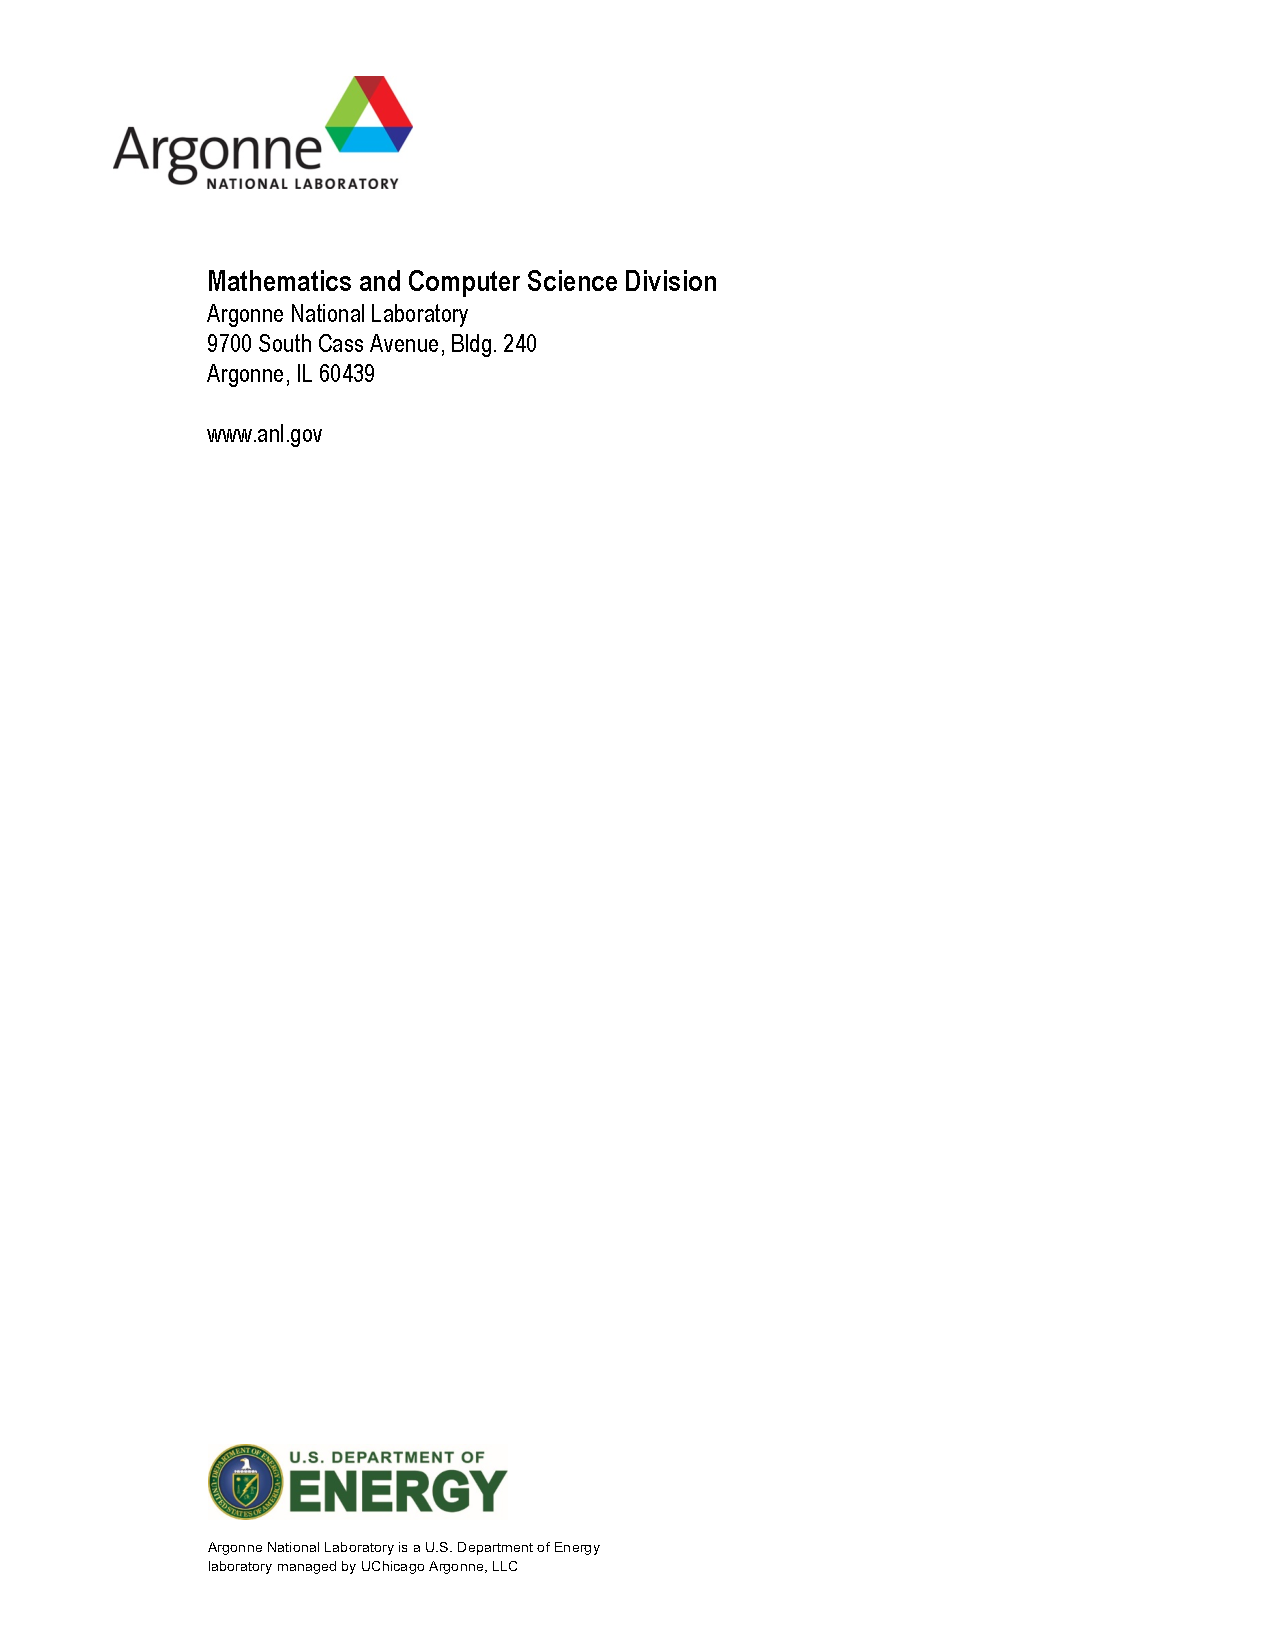
\includegraphics{ArgonneReportTemplateLastPage}}
\restoregeometry

\end{document}


%%% Local Variables:
%%% mode: latex
%%% TeX-master: t
%%% End:
